% siminos/spatiotemp/chapter/Henon.tex
% $Author: predrag $ $Date: 2021-12-24 01:25:20 -0500 (Fri, 24 Dec 2021) $

\Chapter{Henon}{28apr2021}{{\Henlatt}}
% \label{c-Henon}  % formatted for ChaosBook.org


\section{\Henon\ blog}
\label{sect:HenonBlog}

\begin{description}

    \item[2021-02-17 Predrag]
Predrag's  key 2005 result is presumably the time-reversal symmetry
induced, temporal lattice cycle by cycle full square
\refeq{EGfactorSincExcl} and \refeq{EGfactorS}.

    \item[2021-02-15 Predrag]
Added \HenonMap\ examples, mostly for Sidney
(to be edited and returned to ChaosBook):

\refexam{exam:HenonMap}~{\em {\HenonMap}}

% \refexam{exam:cycStabMap}~{\em Stability of cycles for maps}

\refexam{exam:HamHenonMap}~{\em {\Henlatt}}

\refexam{exam:HamHenonJacob}~{\em {\Henlatt} stability}

\refexam{exam:RevHenonMap}~{\em Hamiltonian {\HenonMap}, reversibility}

\refexam{exam:StandMapSymmLin}~{\em Symmetry lines of the standard map}

\refexam{exam:CatMapSymmLin}~{\em Symmetry lines of the cat map}


\end{description}

\subsection{{\Henlatt}; anti-integrable limit}
\label{sect:HamHenonMap}

\begin{description}
  \item[2021-12-23 Predrag]
See also
\refsect{sect:phi4latt}~{\em Classical {$\phi^4$} lattice field theory}

\item[2021-12-22] % Predrag]
\HREF{https://amath.colorado.edu/faculty/jdm/research.html} {Jim Meiss}:
"The concept of anti-integrability was introduced by Aubry and
Abramovici\rf{AuAb90} in 1983 for the standard map (PC: 1983? maybe he
means Aubry and Le Daeron\rf{AuDae83}?), viewed as a linear chain of
particles connected by springs in a periodic potential. They reasoned
that the integrable limit corresponded to vanishing potential energy, so
that the springs dominated giving equal spacing at equilibrium. By
contrast, anti-integrability corresponds to vanishing kinetic energy, so
that particles sit at critical points of the potential. What is most
interesting about this limit is that it is relatively easy, using a
contraction mapping style argument, to show that AI states persist, and
this gives conjugacy to a shift on a symbolic dynamics."

\item[2021-06-04 Predrag]
David Meiss' student David G. Sterling\rf{SterlingThesis99}
much (undeservedly)
un-cited \HREF{https://www.proquest.com/docview/304508605} {PhD thesis},
Univ. of Colorado,
{\em Anti-Integrable Continuation and the Destruction of Chaos} has much
to teach us. He studies \emph{coupled {\HenonMap} lattices} in both
Hamiltonian and Lagrangian formulations; his definition seems pretty much
consistent with our \refeq{SVWhenSTlatt}, though he has a coupling
parameter $c$ used to make spatial couplings weak. The
``anti-integrable'' refers to our choice $a\geq6$, I believe - parameter
regimes in which all of the horseshoe orbits exists.

``Specifying the anti-integrable state for an orbit of a coupled map
lattice requires a multidimensional symbolic object which we call a
symbol tensor.''

His Figures 6.7, 6.18 are reminiscent of my pruning front.

Thesis abstract:
[...] Recurrent phenomena, the
simplest of which is periodic motion, are particularly interesting and
practical objects of study. Scientists have long been captivated by the
near periodic motions of the planets. Among them, \Poincare\ was the
first to truly recognize the importance of periodic solutions in
understanding more complex dynamical behavior. [...] This research has
two complementary aspects. Not only do we develop a technique for
locating periodic orbits in discrete dynamical systems, but we then use
these orbits to study bifurcations, most significantly the global
bifurcation that signals the destruction of chaos. Our technique embodies
the following basic principles:
\\
(1) periodic orbits are conveniently described by a variational principle,
\\
(2) in a special case, the variation principle simplifies, and
\\
(3) continuation from this limiting
case is an effective method for studying periodic orbits. We illustrate
this approach on the \HenonMap.

\item[2021-09-12 Sidney, Predrag]
In the $a\rightarrow\infty$, \emph{anti-integrable} limit\rf{StMeiss98}
the \Henon's original map
\refeq{PCe_ar_pres} goes to $a(\ssp^*)^2=1$,
so
\beq
\ssp_\zeit=\Ssym{\zeit}\ssp^*
    \,,\qquad
\ssp^*=a^{-1/2}
    \,,\quad
\Ssym{\zeit}\in\{-,+\}
\,.
\ee{hen-a-infty}
The small perturbation parameter for the problem is
$\ssp^*=a^{-1/2}$, so replace
\beq
\ssp_\zeit = \Ssym{\zeit}\ssp^* +\hat{\ssp}_\zeit
\,,
\ee{hen-a-infty1}
study the \henlatt\ equations for $\hat{\ssp}_\zeit$.

\item[2021-09-12 Sidney]
The process for perturbations that you're describing sounds very
reminiscent of what is in chapter 11 of Townsend, would that be worth
trying to copy here?

\item[2021-12-22 Predrag]
Moved `generalized {\HenonMap}s' AKA $\phi^4$ field theory posts to
\refsect{sect:phi4latt}~{\em Classical {$\phi^4$} lattice field theory}.

\item[2021-06-04 Predrag]
Read also

Aubry and Le Daeron\rf{AuDae83}
{\em The discrete {Frenkel-Kontorova} model and its extensions.
{I}. {Exact} results for the ground-states} (1983)

Sterling and Meiss\rf{StMeiss98}
{\em Computing periodic orbits using the anti-integrable limit}  (1988)

Aubry and Abramovici\rf{AuAb90},
{\em Chaotic trajectories in the standard map.
{The} concept of anti-integrability},
(1990)

Aubry\rf{aub95ant}
  {\em Anti-integrability in dynamical and variational problems} (1995)

\item[2021-06-04 Predrag]
They are probably deep and good, but I find

Bolotin and MacKay\rf{BolMac97}
{\em Multibump orbits near the anti-integrable limit for {Lagrangian} systems},
(1997)

Bolotin and Treschev\rf{BolTre15}
{\em The anti-integrable limit} (2015)

hard to read. Gave up.


\item[2021-06-04 Predrag]
We all might find the Sect.~III of {Wen's 2014 project}
\wwwcb{/projects/Wen14.pdf} interesting.
\\
Wen says that the original \Henon's\rf{henon} Hamiltonian {\HenonMap} is
equivalent to the harmonic oscillator system. By that he means it can be
interpreted as a kicked driven harmonic oscillator with a nonlinear,
cubic potential kicking term\rf{Heagy92}. If we write anything about \henlatt, we
should include this as a physical motivation.

Check out also Zalmond C. Barney
\HREF{https://fau.digital.flvc.org/islandora/object/fau\%3A3758/datastream/OBJ/view/Derivation_of_planar_diffeomorphisms_from_Hamiltonians_with_a_kick.pdf}
{Master's Thesis}
{\em Derivation of planar diffeomorphisms from Hamiltonians with a kick}.

Butusov \etal\rf{BKPPB18}
{\em Discrete chaotic maps obtained by symmetric integration}
might be of interest for adding a reflection symmetry to the {\HenonMap}.

\item[2021-09-07 Predrag 2 Sidney].

\begin{enumerate}
  \item
Plot lattice field values for $a>>1$, then try to look at a perturbation
theory treatment of this.
  \item
Learn about the
perturbative treatments of field theories.
\end{enumerate}

\item[2021-09-09 Predrag]
Re. 1. above:
I quickly tried to sketch how $a>>1$, did not get anything sensible.
Might be yet another crazy idea that met instant death, do not worry
about it for now.

\item[2021-09-12 Sidney]
% It does work for me now, I'm very sorry about the baby...I'll be more careful in the future.

I did some preliminary calculations of $a>>1$ using the Gallas scaling
(so not quite field theory, but I good test) and as $a$ got larger, the
less variation in lattice site values occurred. There were still
negative, and positive values, but in the large $a$ limit the lattice
site values all approached an equal absolute value. I am not sure if that
is useful, perhaps if we looked at the asymptotic behavior of both large
and small $a$ we could come up with some interesting "asymptotic
\henlatt" theory.

\item[2021-09-12 Predrag]
That sounds very good: in this limit the fields are apparently
$\ssp_\zeit=\Ssym{\zeit}\ssp^*$,
$\Ssym{\zeit}\in\{-,+\}$,
where $-\to0$, $+\to1$ is the binary label corresponding to
lattice site $\zeit$.

Basically you get a theory even simpler than the \templatt.

Perturbation theory for large but finite $a$ would come from replacement
$\ssp_\zeit \to \ssp^*+\epsilon\hat{\ssp}_\zeit$ in the equations,
and ordering terms by powers $\epsilon^k$ and $a^{-\ell}$.
Probably  $a^{-\ell}$ only.

\item[2021-09-12 Predrag]
Do you have the analytic value of $\ssp^*$?

\item[2021-09-13 Sidney]
I have changed my code so that it can be easily switched between
the \Henon\rf{henon} \refeq{PCe_ar_pres}, and Endler and Gallas\rf{EG05}
rescaled \refeq{EG05:ar_pres}, I have added this updated code
\emph{Relaxation Method Henon with Orbit Jacobian.py} to
\emph{siminos/williams/python/relax}.

So, let's see if I understand, if we plug \eqref{hen-a-infty} into the
\Henon\ form \refeq{PCe_ar_pres}, expand and keep only linear terms of
$\hat{\ssp}_\zeit$, we get a new \henlatt\ of form:
\beq\label{pert-henlatt}
\hat{\ssp}_{t+1}+2\Ssym{\zeit}a^{1/2}\hat{\ssp}_\zeit+\hat{\ssp}_{t-1}
    =  %\PCedit{1}
       -(m_{t+1}+m_{t-1})\ssp^*
\,,
\eeq
where $\Ssym{\zeit}$ is determined by the cycle itinerary. Is that the
form you were thinking of? If this is the correct procedure, I can't see
a way of extending this to a second-order perturbation theory, as that is
just reproducing \henlatt.

\item[2021-09-13 Predrag]
I have not thought through your \refeq{pert-henlatt} yet.
Maybe $\hat{\ssp}_\zeit\to\ssp^*\hat{\ssp}_\zeit$ helps a bit.

You have analytic formulas for fixed points \refeq{COM:eq2}, period-2
{\lattstate}s \refeq{COM:2-cycle}. You might find useful approximate
large $a$ formulas for all period-\cl{}\ {\lattstate}s.
They might already be in David Sterling's %\rf{Sterling99}
\HREF{https://www.proquest.com/docview/304508605} {PhD thesis}.

Maybe {\HillDet}s have interesting expansions in powers of
$a^{-\ell/2}$...


\end{description}


For the contraction parameter value
 $b=-1$ the \HenonMap\rf{henon} is orientation and area
preserving, and can be written as a 3-term recurrence
relation
\beq
  x_{\zeit-1} = 1-ax_\zeit^2-x_{\zeit+1}
\,.
\ee{PCe_ar_pres}
Multiply both sides by $-2a$ and define the  \Henon\ `field' at lattice
site $\zeit$ to be $\ssp_\zeit=-2ax_\zeit$. We shall refer to this form
of \Henon\ as the {\em \henlatt}:
\beq
\ssp_{\zeit+1} - \frac{1}{2}\ssp_{\zeit}^2 +\ssp_{\zeit-1}=-2a
\,.
\label{Hen-1dLatt}
\eeq
or we can multiply both sides by $-2$ and define the  \Henon\ `field' at lattice
site $\zeit$ to be $\ssp_\zeit=-2x_\zeit$, yielding {\henlatt} of form:
\beq
\ssp_{\zeit+1} - \frac{a}{2}\ssp_{\zeit}^2 +\ssp_{\zeit-1}=-\Ssym{\zeit}
\,,\quad
\Ssym{\zeit}=2
\,,
\label{Hen-1dLattA}
\eeq
with the `coupling constant' $a$ the analogue of the stretching factor
${s}$ in \templatt\ \refeq{LC21:catMapNewt}, and a constant source
$\Ssym{\zeit}$.

The fixed points $\ssp_j=\ssp$ satisfy
\beq
\ssp^2 - \frac{4}{a}\,\ssp - \frac{4}{a} =0
\,,\qquad
\ssp_\pm =  \frac{2}{a} \pm \sqrt{ \frac{4}{a^2}+  \frac{16}{a}}
\label{Hen-1dLattFix}
\eeq




{\Henlatt} is $\phi^3$ lattice field theory.
Biham-Wenzel\rf{afind} find \Henon\ {\lattstate}s by constructing a cubic
action density \refeq{BWcubic},
\beq
S[\ssp]_\zeit - \Ssym{\zeit}\,\ssp_\zeit
      =  \ssp_{\zeit+1}\ssp_\zeit + \ssp_\zeit\ssp_{\zeit-1}
         -\frac{a}{3!}\ssp_\zeit^3
         - \Ssym{\zeit}\,\ssp_\zeit
\,,\qquad
\Ssym{\zeit}=2
\,.
\ee{henlattBWcubic}

Still to check: is $\Ssym{\zeit}=\pm2$ the Biham-Wenzel method?
Looks like it, as that amounts to flipping the sign of the cubic term
while keeping the variation across there sits of the same magnitude.

I took $+2\ssp_n$ out of $S[\ssp]$ to treat it as a source density term
$\Ssym{\zeit}\ssp_\zeit$.

Now the {\jacobianOrb} \refeq{jMorb1dField} is of the same form as the \templatt\
{\jacobianOrb} \refeq{LC21:Hessian},
\beq
\jMorb[\Xx] =
\left(\begin{array}{cccccccc}
%\begin{pmatrix}
 {s}_{0} &-1 & 0 & 0 & \cdots & 0 & 0 &-1 \\
      -1 & {s}_{1} &-1 & 0 & \cdots & 0 & 0 & 0 \\
       0 &-1 &  {s}_{2} &-1 & \cdots & 0 & 0 & 0 \\
  \vdots & \vdots & \vdots & \vdots & \ddots & \vdots & \vdots & \vdots \\
       0 & 0 & 0 & 0 & \cdots &-1 &  {s}_{\cl{}-2} &-1 \\
      -1 & 0 & 0 & 0 & \cdots & 0 &-1 &  {s}_{\cl{}-1}
%\end{pmatrix}
          \end{array} \right)
\,,
\ee{jMorb1dField} %was {PCJiKoKr20(8)}
%
but with the stretching factor at site $\zeit$ depending on
the particular \lattstate, ${s}_{\zeit}=\ssp_{\zeit}$,
and once you have an expression for  \HillDet\ $\|\jMorb[\Xx]\|$ in terms of traces
$\Tr\jMorb^k$ ,
\ie, the $\Dn{\cl{}}$ invariant
orbital sums for products of fields on consecutive lattice sites,
they will be the same for the \templatt\ and the \henlatt.

\section{{\HenonMap} symmetries}
\label{s-HenonSymm}
% 2021-02-15  Predrag if edits, return to appendFiniteGr
\index{Henon@H\'enon map!symmetries}
\index{symmetry!H\'enon map}
\index{map!H\'enon}

We note here the symmetries of the {\HenonMap}
\refeq{eq2.1a}.
For $b \neq 0$ the  {\HenonMap} is reversible:
the backward iteration of \refeq{2-step} is given by
\beq
  x_{n-1} = -\frac{1}{b} (1-ax_n^2-x_{n+1})
\,.
\ee{e_henon_inv}
Hence the time reversal amounts to $b \rightarrow 1/b$,
$a \rightarrow a/b^2$ symmetry in the parameter plane, together
with $x \rightarrow -x/b$ in the coordinate plane, and there is
no need to explore the $(a,b)$ parameter plane outside the strip
$b \in \{-1, 1\}$.
For $b=-1$ the map is orientation and area preserving
Hamiltonian {\HenonMap} %\refeq{e_ar_pres}
% restore     \PublicPrivate{,}{% switch \PublicPrivate{
% restore     (see \refeq{} below),
% restore           }% end \PublicPrivate{
% restore     \PC{define orientation, area preserving}
\index{orientation!preserving map}
\index{map!orientation preserving}
\index{area preserving!map}
\index{map!area preserving}
\beq
  x_{n-1} = 1-ax_n^2-x_{n+1}
\,,
\ee{e_ar_pres}
the backward and the forward iteration are the same, and the \nws\ is
symmetric across the $x_{n+1} = x_n$ diagonal. We can write this as a
nonlinear field equation with a Laplacian \refeq{Box(2.1.1)} and a
``cubic'' potential \refeq{BWcubic}
\beq
  % x_{n-1}-2\,x_{n}+x_{n+1}
\Box\,x_{n}+(a\,x_{n}+2)\,x_{n}\,=\, 1
\,.
\ee{HenonLapl}
% restore     \PC{define the \orev\ case}
Endler and Gallas\rf{EG05} prefer the equivalent, rescaled form
\refeq{EG05:ar_pres}.

This is one of the simplest models of a \PoincMap\ for a Hamiltonian flow.
\index{Hamiltonian!flow}
\index{flow!Hamiltonian}

For the \orev\ $b=1$ case we have `golden \Henon' (in analogy with \refeq{goldenCat})
\index{orientation!reversing map}
\index{map!orientation reversing}
\beq
  x_{n-1} = 1-ax_n^2+x_{n+1}
\,,
\ee{e_ar_rev}
and the \nws\ is symmetric across the $x_{n+1}=-x_n$ diagonal.

  % siminos/spatiotemp/Solutions/soluCOM.tex
% $Author: predrag $ $Date: 2021-12-24 01:25:20 -0500 (Fri, 24 Dec 2021) $

% Predrag soluCOM.tex                                           2021-02-15
%               ChaosBook.org soluCOM.tex   to here
%predrag                24mar2005
%predrag                24jan2005
%predrag                 3jan2005
%predrag                27dec2004

\section{``Center of mass'' puzzle}
\label{s:CenterOfMass}
\index{center of mass}

Some of Predrag's unpublished 2004 drafts and calculations are in
\begin{verbatim}
% dasbuch/book/FigSrc/gnu/Gallas % just a link
dasbuch/WWW/library/Gallas-chiral.pdf
dasbuch/WWW/projects/revHenon/Gallas0101305.txt  etc
dasbuch/book/Fig/COM0001011.eps  COM0001101.eps  COM000111.eps
                 COM0011.eps     COM011.eps
dasbuch/book/OldProblems/soluCOM011005.tex
\end{verbatim}

\noindent
{\em predrag/reports/referee/Gallas.txt} on the unpublished

{\em Periodic orbits are not necessarily independent from each other}

\noindent
Some of Predrag's unpublished 2004 drafts and calculations
of Jan 26, 1999 suggests many references where similar work was
published. The revised paper appeared as Gallas\rf{Gallas99} {\em
Nonlinear dependencies between sets of periodic orbits}, I believe.
\\

 {{\em Gallas-chiral.pdf}} \CBlibrary{Gallas-chiral} has the Endler-Gallas
\HenonMap\ polynomials up to period 8, and nothing else.
\\

\wwwcb{/projects/revHenon} has lots of stuff:
\begin{enumerate}
  \item
\emph{chiral.pdf} is an unfinished draft of Endler, Gallas and
Cvitanovi{\'c} paper, based on {\em Gallas-chiral.pdf}. Much of the
introduction is utterly delirious. Notation for `orbits', eq.~(10)
is redundant and the indices of $x_j$ are useless, they label roots of
different polynomials, ordered by increasing $x_j$.

Figures illustrate `chiral' orbit pairs, $A_\cl{}=0$;
 $B_\cl{}=0$ and  $C_\cl{}=0$ self-dual orbits. Fig.~4 might be
$C_\cl{}=0$ for value of $a$ other than 6.

  \item
From: Jason Alfredo Carlson Gallas (14 Jan 2005) fortran \emph{plot\_orbit.f},
generates *.eps files, see \emph{Fig-7cycles.txt},
\emph{Gallas0101305.txt}.

  \item
{\em per7.pdf} 18 period-7 orbits.

  \item
{\em chiral\_p8.pdf} 3 period-8 time-asymmetric pairs.

  \item
{\em per8.pdf}: 18 self-dual period-8 orbits (not sure that is a
complete list).

  \item
{\em FourClasses.pdf}: defines four classes of orbits under time reversal;
perhaps useful, still need to find the LaTeX file.

  \item
{\em tres.pdf}: period-6, symmetries with respect to the main diagonal
of 3 6-cycles ``corresponding to a $\sigma^3$ factor,'' plotted for $a=7$.
No idea what that is...

  \item
\emph{Gallas0101305.txt} says he does not understand me.

  \item
\emph{Predrag011304.txt}  my last attempt to explain symbolic dynamics
and why is this a time-reversal symmetry. ``Please use `time reversal'
rather than `chiral'. It is a standard part of the lore of Hamiltonian
dynamics, and especially Hamiltonian/symplectic mappings.'' Hopeless.

  \item
{\em puzzle.pdf}, {\em puzzle.tex} is January 25, 2005 version of Endler and
Gallas\rf{EG05} (submitted December 25, 2005?) that uses ChaosBook
notation - Table~1 can be used as a check on Sidney's \po s.
Other versions:
{\em puzzle011305.tex}  of 13 Jan 2005;
 {\em puzzle.tex} and {\em puzzle2dasbuch.tex} of 27 Jan 2005;

They published in {\em Reductions and simplifications of
orbital sums in a {Hamiltonian} repeller}\rf{EndGal06} without me as a
coauthor. Algebraic number expressions for periodic points
show interesting patterns, their eqs.~(22),
(23) and (28), that would not be noticed from their numerical values.

They use binary labelling also in Endler and Gallas\rf{EG05a} {\em
Conjugacy classes and chiral doublets in the {H{\'e}non Hamiltonian}
repeller}, without mentioning me or ChaosBook at all.

  \item
{\em citation.txt} and {\em puzzle.end} is the footnote which Gallas
would not accept:
{\em endnote27}~~{\em This exact equation was discovered by P.
Cvitanovi\'c during discussion and in collaboration with the authors. }

  \item
{\em old/puzzle011805.pdf} has my comments

  \item
{\em solRevHen.pdf} is extracted from
\wwwcb{/projects}, version 11.2.2, Mar 10 2005. I believe all that is
in ChaosBook, ignore.

  \item
{\em revHenon.pdf}, {\em revHenon.zip} is a template for a
\wwwcb{/projects} extracted from Jason Gallas, Predrag edited \emph{puzzle.tex},
Gallas text	removed 18 Feb 2006.
I believe no one took up the project.
\end{enumerate}

To summarize, this 2005 work agrees with current Han's work, but does not
clarify the problems we are dealing with now. The figures might be useful
as crosschecks for Sidney's \Henon\ orbits.

\bigskip

\begin{description}
\item[2021-02-16 Predrag]
% in ChaosBook.org \solution{e:CenterOfMass}{``Center of mass'' puzzle$^{**}$.}{
\PC{27dec2004}{
Extracted from the ChaosBook.org boyscout,  version of 2018-08-02 tex files.
Edited here, so eventually return to ChaosBook.
}
                                                        \toCB
Here are my notes on the work of Gallas and collaborators;
they have written many papers on
polynomial maps%
\rf{EndGal01,EndGal02,EG05,EG05a,EndGal06,Gallas18,Gallas20,Gallas20a}.
What I had contributed (unpublished, I believe) is to show Gallas
how to use time-reversal,
\refeq{EGfactor2B}, \refeq{EGfactorS} and \refeq{EGfactorP},
wrote a draft of a paper (click on
\HREF{Http://ChaosBook.org/projects/revHenon/chiral.pdf} {chiral.pdf}),
and --when he was not interested in it-- requested my traditional citation,
\begin{quote}
 This exact equation was discovered by P. Cvitanovi\'c
during discussion and in collaboration with the authors.
\end{quote}
but he refused to credit me for that, so I - what's the point - I stopped
following their papers. I remember him being stubborn in a male kind of
way. Absolutely refuses to understand binary symbolic dynamics, that what
he understands\rf{gallas_counting} to be `spatial $x\leftrightarrow{y}$
symmetry'

\begin{quote}
``[...] three algebraic conjugacy classes with respect to
a spatial reflection $R(x, y) = (y, x)$ about the $y = x$ symmetry
diagonal in phase-space.''
\end{quote}

is time reversal, and he would not try to understand ChaosBook symmetry
factorizations.  But it is quite possible that they (or younger me?) did
the right thing and quotiented the time reversal... Check the papers and
the papers they refer to.

As he has worked on this for at least 20 years, there are many details
specific to quadratic mappings that I think we can ignore here. Here is
an overview from my point of view:
Gallas \etal\ observe that
\begin{enumerate}
  \item
for polynomial mapping \refeq{cycle-polyn} the \emph{orbital sum}
\beq
\sigma_p = \sum_{i \in p} x_{p,i}
\ee{COMdef}
% \refeq{COMdef}
is a \emph{prime} cycle $p$ \emph{invariant} that satisfies a
(factorized!) polynomial equation
${\mathbb S}_\cl{}(\sigma)=0$
of the order $\cl{p}$, the period of the cycle, see for example
\refeq{Gallas20a:S_5}.

{\bf Predrag addendum}:
{\HillDet}s are \emph{symmetric polynomials} in lattice fields
$\{\field_1,\field_2,\cdots,\field_\cl{}\}$, which are, by construction,
all \emph{prime} cycle $p$ \emph{invariants}.
The {orbital sum} \refeq{COMdef} is one example.
Another one is the bilinear \refeq{HillDetHen2cycle}.

  \item
the cycle-points $\ssp_{p,i}$ of a given cycle are roots of a polynomial
\refeq{cycle-polyn} of order  $\cl{p}$, see for example
\refeq{Gallas20a:c_5,1}. This is remarkable, as higher iterates of a
polynomial mapping are polynomials of a horrendous order.
  \item
time-reversal invariance (my interpretation, not theirs) induces the
\beq
{\mathbb S}_\cl{} = C_\cl{}^2 D_\cl{} N_\cl{}
\,.
\ee{EGfactorS}
factorization of such polynomials, where D=`diagonal'
class, N=`non-diagonal' class, and `C=`chiral' class, see below.

For me this is the key result.
\end{enumerate}

This ${\mathbb S}_\cl{}$ is very smart, as it has a zero for every
\emph{prime} orbit. Perhaps we can bring this to a full square, by
including the boundary into the definition of the temporal lattice
fundamental domain, with $(C D N)$ {\orbit}s (perhaps in the Fourier
space - they talk about `cyclotomic polynomials')
\beq
{\mathbb S} = \frac{(C D N)^2}{D N}
\ee{EGfactorSincExcl}
by taking care of the temporal fundamental domain boundary by the
inclusion-exclusion principle \refeq{KlaRot97(2.1)}, and proceed to
zeta-function factorization in the spirit of \refeq{Lat-LapSqrt},
\refeq{tildejMorbRel}, for each { Hamiltonian {\Henon}} cycle separately.

I believe factorization \refeq{EGfactorSincExcl} should apply to
\po s of \emph{any time-reversible} mapping, not just \Henon\ and \templatt,
but the `N class' worries me.

 \refeq{Lat-LapSqrt}

\bea
\left(\shift-\unit\right)
 &=&
\tilde{\shift}\tilde{\partial}
     % \left(\tilde{\shift}-\tilde{\shift}^{-1}\right)
    \continue
\left(\shift^{-1}-\unit\right)\left(\shift-\unit\right)
 &=&
    - \tilde{\partial}^2
  = \Box
    %\left(\tilde{\shift}-\tilde{\shift}^{-1}\right)^2
 \label{COM:LapSqrt}\\
\jMorb  &=& \Box - \mu^2\unit
         =
\left(
\tilde{\partial} + \mu\unit  %\left(\tilde{\shift}-\tilde{\shift}^{-1}\right)
\right)
\left(
\tilde{\partial} - \mu\unit  %\left(\tilde{\shift}-\tilde{\shift}^{-1}\right)
\right)
    \continue
\tilde{\jMorb}
     &=& \tilde{\partial} - {\mu}\unit
    \,=\,
    \tilde{\shift} - \mu\unit -\tilde{\shift}^{-1}
\nnu
\eea


\item[2021-02-19 Predrag]
Gallas\rf{gallas_counting} {\em Counting orbits in conjugacy classes of
the {{\Henon} Hamiltonian} repeller} counts the numbers $C_\cl{}$,
$D_\cl{}$, $N_\cl{}$ of \refeq{EGfactorSincExcl} {\orbit}s
(switched to calling `prime cycles' orbits, like Gallas does) in each class, for any
arbitrary period $\cl{}$.

$D_\cl{}$ is sensible, relatively simply related to the number of points on the
time-reversal diagonal; one expects something like that for any system.

 $N_\cl{}$ is funky,  has to do with the parabola symmetry
line, might be what we call "dynamical".

$C_\cl{}$ is just the remainder $M_\cl{}-D_\cl{}-N_\cl{}$:
$C_1=\cdots=C_5=0$, and then (Gallas Table~1), starting with $C_6/2=1$:
\beq
  1,2,6,14,30,62,127,252,500,968, 25446,\cdots
\ee{gallas_counting:tab1}
This is not in \emph{On-Line Encyclopedia of Integer Sequences}
\HREF{https://oeis.org/} {OEIS},
(It is close to \HREF{https://oeis.org/A000918} {OEIS:A000918} A000918 		
$a(n) = 2^n - 2$ and $a(n+1) = 2 + 2a(n)$)
so it has to be reverse engineered to find the $\tilde{N}_\cl{}$, the numbers of
periodic points of the yet to be written down $\sqrt{\mbox{\Henon\ map}}$.


The number of $C_\cl{}/2$ periodic points:
\[
  \tilde{N}_6= 1*6=6,
  \tilde{N}_7= 2*7=14,
  \tilde{N}_8= 6*8=48,
  \tilde{N}_9= 14*9=126,
\]
Actually, $ \tilde{N}_\cl{}= \cl{}\,C_\cl{}/2+\cl{}(D_{2\cl{}}+N_{2\cl{}})$
looks more sensible
\[
  \tilde{N}_6= **,
  \tilde{N}_7= 2*7+1=5,
  \tilde{N}_8= 6*8+1=19,
  \tilde{N}_9= 14*9+2*2+1=61,
\]


MacKay had these numbers already
listed in Table 1.2.3.5.1 of his 1982 PhD thesis\rf{Bmack93}
\CBlibrary{Bmack93}.

%%%%%%%%%%%%%%%%%%%%%%%%%%%%%%%%%%%%%%%%%%%%%%%%%%%%
\begin{table}
\begin{tabular}{c|rrrrr|rrrrr|rrrrr}
$\cl{}$ &  1 &  2 &  3 &  4 &  5 &
       6 &  7 &  8 &  9 & 10 &
      11 \\%& 12 & 13 & 14 & 15 \\
\hline
$N_\cl{}$ &  2 &  4 &  8 & 16 &  32 &
       64 &  128 &  256 & 512 & 1024 &
      . % \\%& 12 & 13 & 14 & 15 \\
             \rule[-1ex]{0ex}{3.5ex} \\
$M_\cl{}$ &   2 &   1 &   2 &  3 &  6 &
         9 & 18 &  30 & 56  & 99 &
       186 &  %% &     &     &
\end{tabular}
\bigskip
\caption{\label{tab:HamHenon}
{\Lattstate}s and %{prime}
orbit counts for the ${a}=6$ \Henon\ map.
Compare with the golden (Fibonacci\rf{BaNeRo13}) cat map \reftab{BaRoWe08fib-tab}
and \refeq{zetasqrt-N}.
}
\end{table}
%%%%%%%%%%%%%%%%%%%%%%%%%%%%%%%%%%%%%%%%%%%%%%%%%%%%
%

%%%%%%%%%%%%%%%%%%%%%%%%%%%%%%%%%%%%%%%%%%%%%%%%%%%%
\begin{table}
\begin{tabular}{c|rrrrr|rrrrr|rrrrr}
$\cl{}$ &  1 &  2 &  3 &  4 &  5 &
       6 &  7 &  8 &  9 & 10 &
      11 & 12 & 13 & 14 & 15 \\
\hline
$\tilde{N}_\cl{}$ &   2 &   2 &   4 &   4 &   8 &
         8 & 16 &  16 & 32 &  32 &
        . & . & . & . & . \rule[-1ex]{0ex}{3.5ex} \\
$\tilde{M}_\cl{}$  &  3 &   . &   . &   . &    . &
             &   . &   . &   . &   . &
           . &  . &   . &   . & .
\end{tabular}
\bigskip
\caption{\label{goldenHen}
    Temporal {\lattstate}s and %{\orbit} counts for the
    $\mu=1$  golden cat map.
    See \refeq{zetasqrt-N} and the counting of walks on
    the ``half time-step'' Markov graph \reffig{fig:HLHalfStepMarkov}.
    }
\end{table}
%%%%%%%%%%%%%%%%%%%%%%%%%%%%%%%%%%%%%%%%%%%%%%%%%%%%


Assuming that \refeq{tildejMorbRel} applies, we can compute
$\tilde{N}(\mu)_{\cl{}}$ from ${N}(s)_{\cl{}}$
\bea
2^n &=& \tilde{N}(\mu)_{\cl{}}^2
    \,,\quad
n \mbox{ odd}
    \continue
2^{\cl{}} &=& \tilde{N}(\mu)_{2\cl{}}
    \,,\quad
n \mbox{ even}
\,.
\label{tildejMorbRelHen}
\eea


\item[2004-12-27 Predrag]
These extracts from ChaosBook.org are meant to complement and perhaps add
to the Endler and Gallas explanation\rf{EG05} of the ``center of mass''
puzzle for the cycles listed in \reftab{gv:cycles}, first observed
numerically by G.~Vattay in \refref{BCISV93}.

\item[2016-09-19 Predrag]
    \PC{2021-02-15} {Copied from {\em DBblog.tex} - return eventually,
    as there are edits here. Not sure where the next few paragraphs came from.}

We present exact formulas solving the problem of partitioning the total
number $M_k$ of period-k orbits of the area-preserving {\HenonMap} into the
number of orbits building its three possible conjugacy classes. The
formulas are valid for any arbitrary period n. They are derived with
combinatorial methods, by an application of the
number-theoretic Moebius inversion formula to a key problem in physics and
dynamical systems. A handy MAPLE implementation of the formulas is also
provided.

A number of orbital symmetries and asymmetries computed analytically and
systematically for the Hamiltonian (area-preserving) $b=-1$ limit of the
{\HenonMap}
have been studied in \refrefs{EG05a,EndGal06}.

Endler and Gallas\rf{EG05} prefer the equivalent, rescaled form $x\to x/a$
of the Hamiltonian {\HenonMap} \refeq{HenonLapl}:
\beq
  x_{n-1} - 2 x_n + x_{n+1} +  (x_n + 2) x_n = a
\,,
\ee{EG05:ar_pres}
They write:
``
The advantage of this equation is that it generates \emph{monic} minimal
polynomials, i.e. polynomials having 1 as the leading coefficient.
''

The key result
reported was the existence of a natural segregation of all orbits into
three algebraic conjugacy classes   with respect to a spatial reflection
R(x,y)=(y,x) about the y=x symmetry diagonal in \statesp. Under
reflection, every periodic orbit was found to fall into one of
three classes:
\begin{itemize}
  \item[D]
diagonal class, formed by symmetric orbits with points on the
time-reversal symmetry diagonal.
An odd period symmetric cycle has an odd number of points on the boundary,
see \reffig{COMcycles}\,(a).
An even period symmetric cycle has an even number of points on the boundary,
see \reffig{COMcycles}\,(b).
  \item[N]
non-diagonal class, formed by self-symmetric orbits without   points on
the symmetry diagonal, see \reffig{COMcycles}\,(c).
  \item[C]
chiral class, formed by pairs of asymmetric cycles that map into each
other, see \reffig{COMcycles}\,(d,e).
\end{itemize}

%%%%%%%%%%%%%%%%%%%%%%%%%%%%%%%%%%%%%%%%%%%%%%%%%%%%%%%%%%%%
% Date: Thu, 13 Jan 2005
% From: Predrag Cvitanovic <predrag.cvitanovic@physics.gatech.edu>
% To: Jason Alfredo Carlson Gallas <jgallas@if.ufrgs.br>
\FIG{
(a)
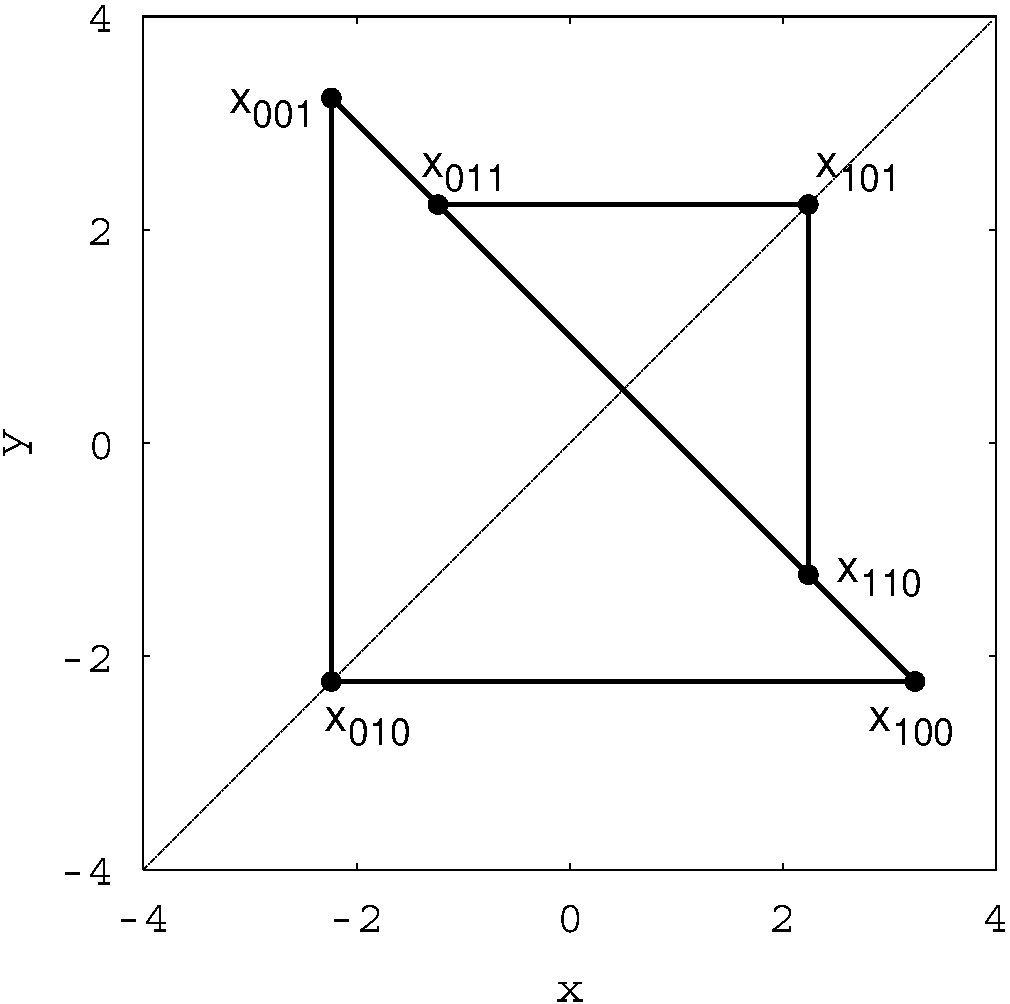
\includegraphics[width=0.30\textwidth]{COM011}
 \;
(b)
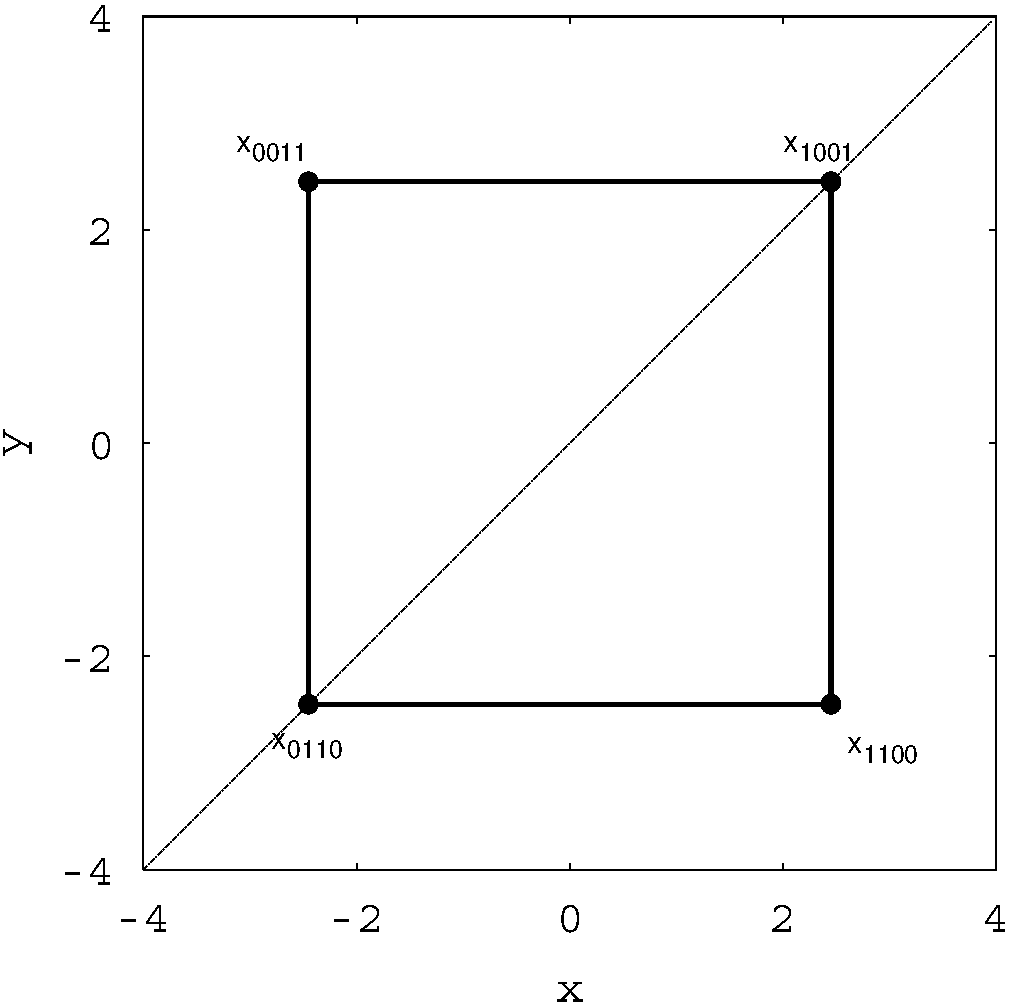
\includegraphics[width=0.30\textwidth]{COM0011}
 \;\\
(c)
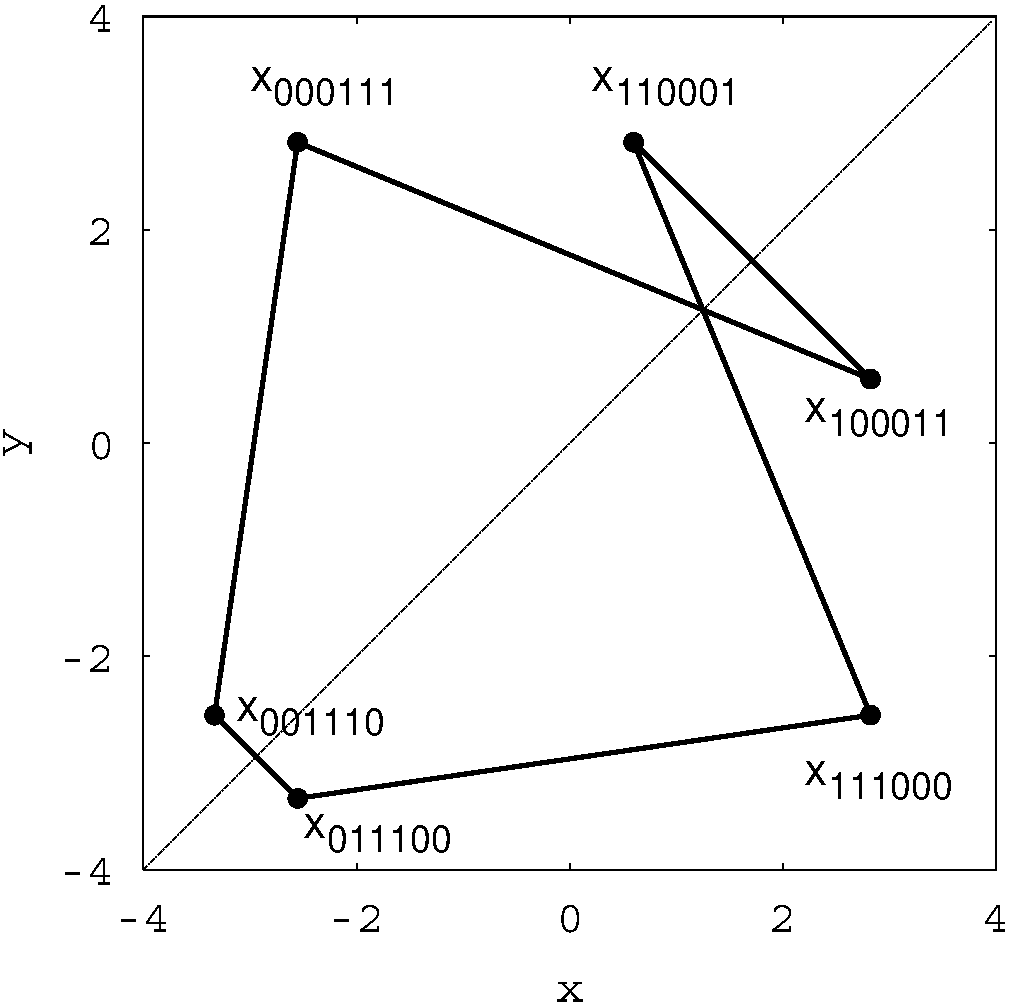
\includegraphics[width=0.30\textwidth]{COM000111}
\\
(d)
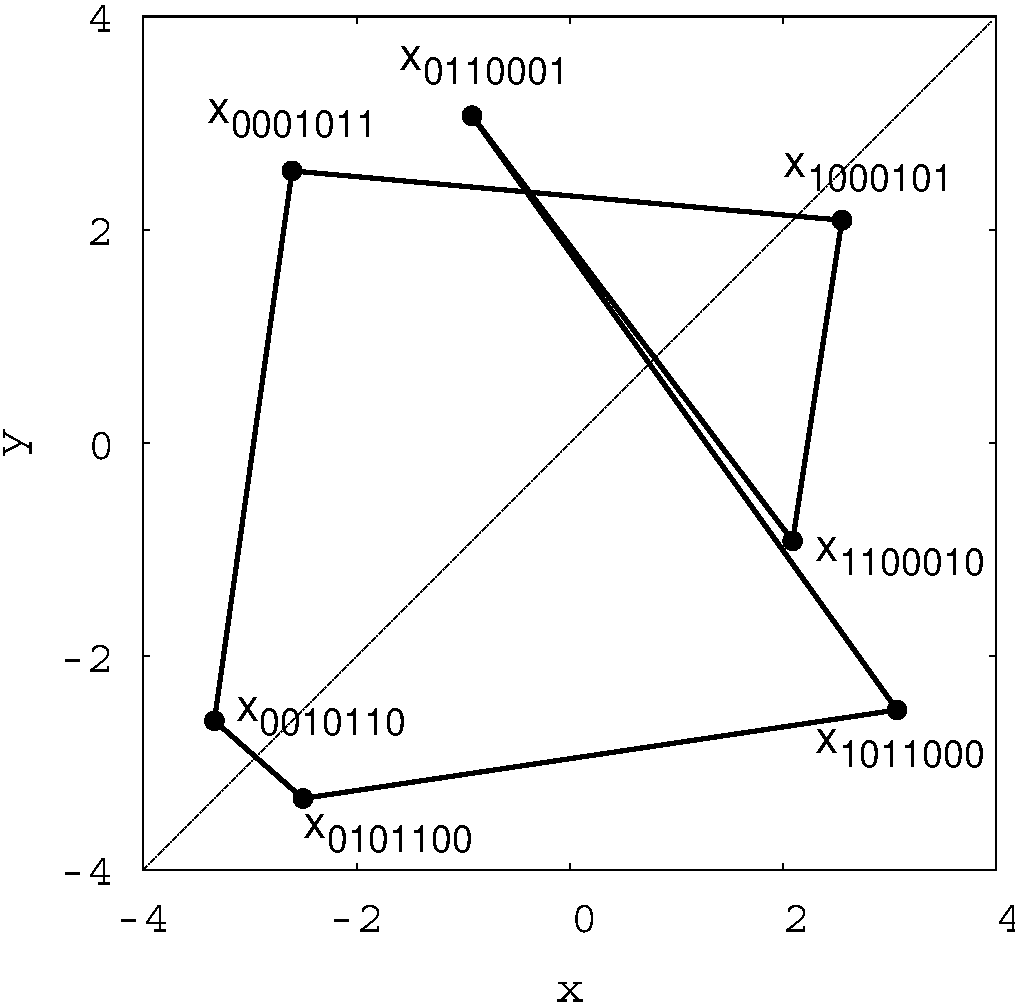
\includegraphics[width=0.30\textwidth]{COM0001011}
 \;
(e)
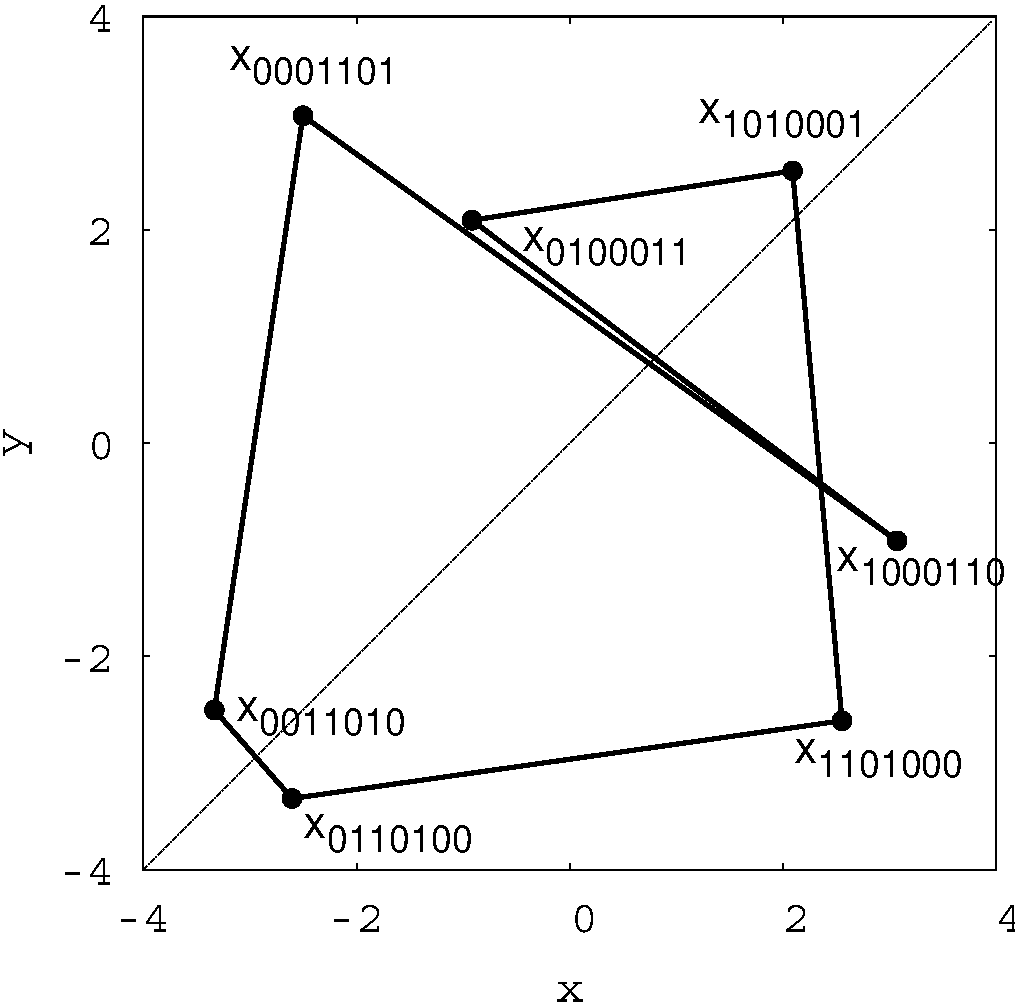
\includegraphics[width=0.30\textwidth]{COM0001101}
}{}{
\Po s of the Hamiltonian {\HenonMap} \refeq{e_ar_pres}:
(a)
An odd-period orbit can have a point on the boundary, and thus belong to the
diagonal class D. Example: the 3-cycles \cycle{001}, \cycle{011}.
(b)
An even-period orbit can have two points on the boundary, and thus belong to the
diagonal class D. Example: the 4-cycle \cycle{0011}.
(c)
An even-period orbit can belong to the non-diagonal class N.
Example: the 6-cycle \cycle{000111}, with no points on the boundary.
(d)
Almost all longer orbits are asymmetric, `chiral' class C.
Example: the 7-cycle \cycle{0001011}, and
(e)
its partner \cycle{0001101} under flip across the diagonal and
time-reversal. Under the time reversal periodic points symbol sequences
are mirrored into their symmetry partners point by point.
For \catlatt\ examples, see
\reffig{fig:HLPeriodicOrbitsA},
\reffig{fig:HLPeriodicOrbitsB},
\reffig{fig:HLSymmetric4CyclesA},
\reffig{fig:HLSymmetric4CyclesB},
\reffig{fig:HLAllCyclePoints}.
}{COMcycles}
%%%%%%%%%%%%%%%%%%%%%%%%%%%%%%%%%%%%%%%%%%%%%%%%%%%%%%%%%%%%%

Each class contains a characteristic algebraic signature embodied by a
specific orbital decompositions (factorizations)\rf{EG05a}. The orbital
segregation is independent of the control parameters and is specially
interesting for $a_h >5.69931\cdots$, the value beyond which there is a
complete Smale horseshoe and all orbits are real.
This Letter  reports exact analytical expressions
that count the numbers $C_n$, $D_n$, $N_n$ of
orbits in each class, for any arbitrary period $n$.

%%%%%%%%%%%%%%%%%%%%%%%%%%%%%%%%%%%%%%%%%%%%%%%%%%%%%%%
\begin{figure}
  \centering
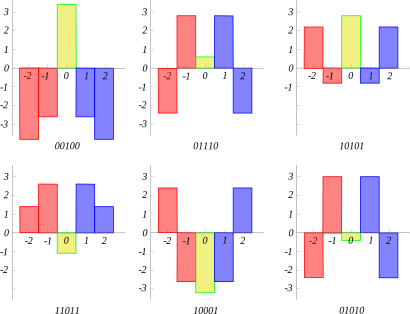
\includegraphics[width=0.95\textwidth]{PChenlatt5cyc} % from HL1dLattRefl0.svg
~~~~~~~~
% 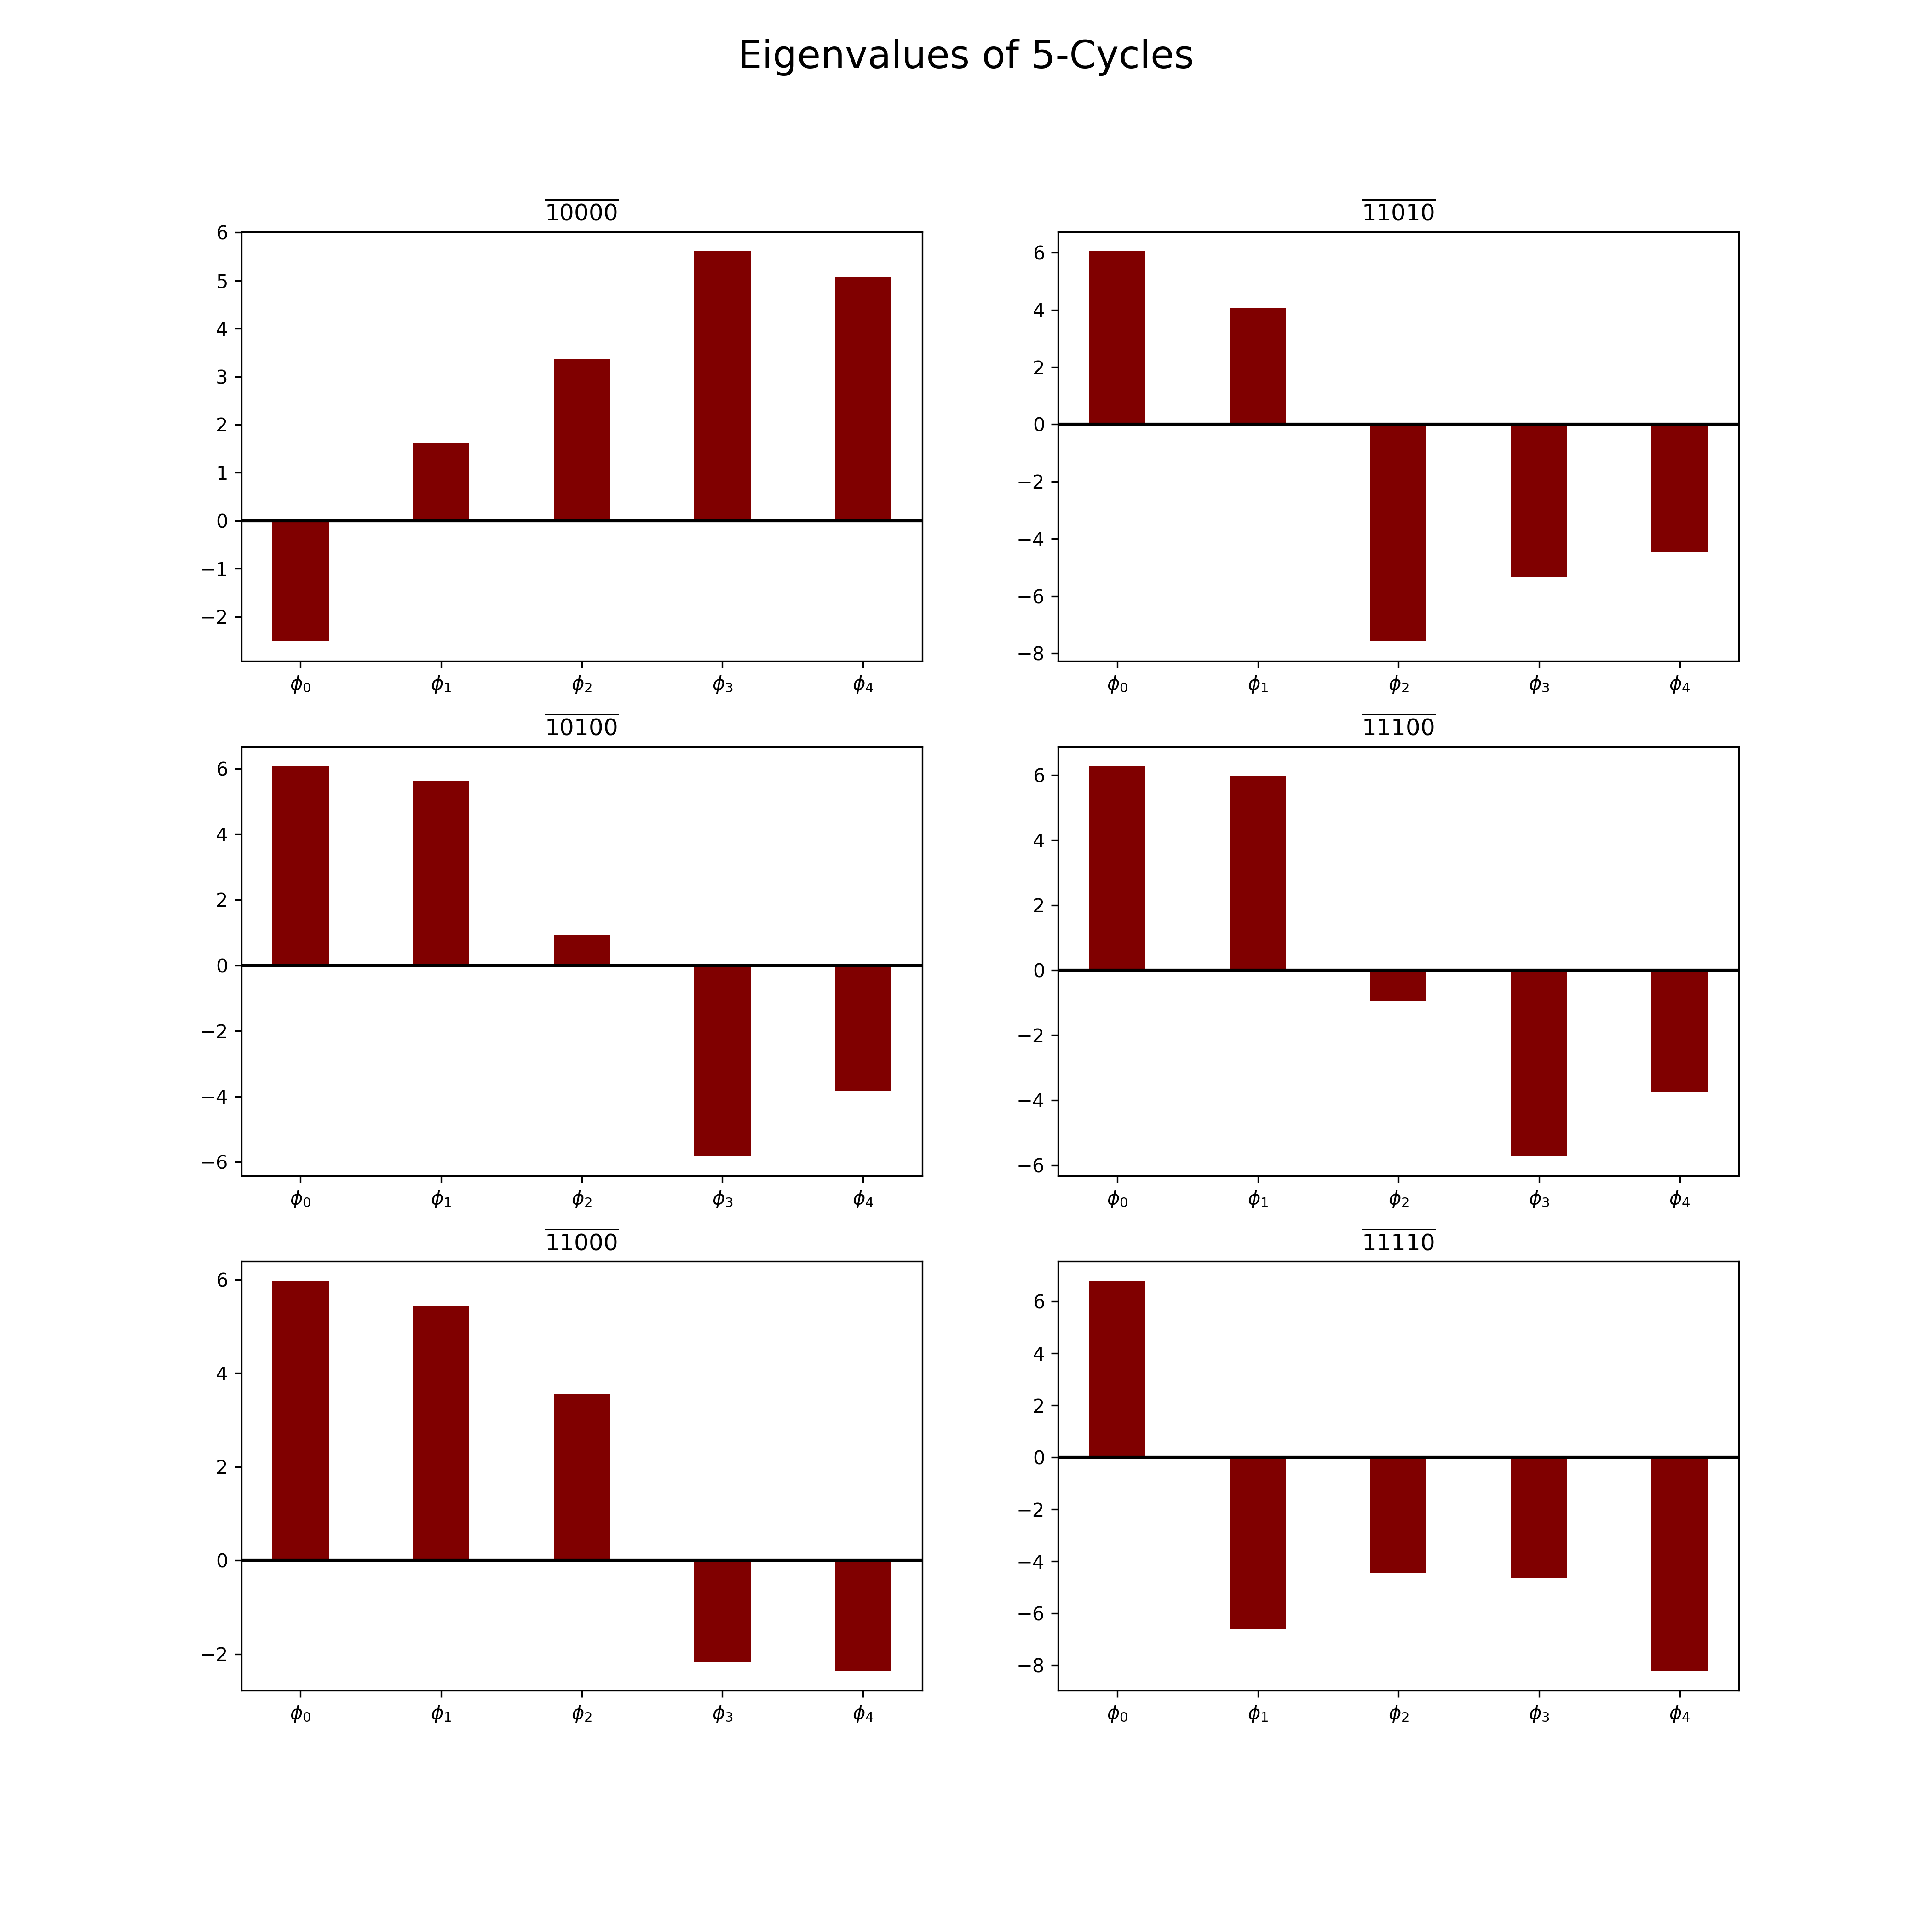
\includegraphics[width=0.45\textwidth]{SVW5eigen}
  \caption{
\Henlatt\ \refeq{Henlatt-2-step}, $a=6$:
Odd period \refeq{reflSymOdd} $\cl{}=5$ {\lattstate}s
$
\cycle{\ssp_{-2} \ssp_{-1} \sitebox{\ssp_0}\,\ssp_1 \ssp_2 |}
$
of \reftab{tab:HenCycD5},
plotted as in
\reffig{fig:symmLattStates}.
Compare also with forward-in time plots of \reffig{fig:EG05aCyc5}.
They are all reflection symmetric, with
the fixed lattice field $\sitebox{\ssp_0}$ colored gold. Note that the
symbolic dynamics is given by the signs of lattice site fields.
The most striking feature of these {\lattstate}s is how far is $a=6$
\henlatt\ from a $0\leftrightarrow1$ symmetry: stretching close to
$\cycle{0}$ constant {\lattstate} is much stronger than close to the
almost marginal $\cycle{1}$ constant {\lattstate}. Probably for somewhat
lower bifurcation value of $a$ than the `critical' value
$a_h=5.69931\cdots$, the fixed lattice sites $\sitebox{\ssp_0}$ for
$\cycle{01110}$ and $\cycle{01010}$ coalesce and vanish, so the
bifurcation happens on the even symmetry site.
{\color{red}If anybody ever gives some thought to {\jacobianOrb}
eigenvalues of \reffig{SVW5CycHamHen}\,(right), the corresponding
eigenvectors might illuminate this point.} As $a\to\infty$ I expect this
symmetry to be restored.
}
\label{fig:PChenlatt5cyc} % started with {SVW5CycHamHen}
\end{figure}
%%%%%%%%%%%%%%%%%%%%%%%%%%%%%%%%%%%%%%%%%%%%%%%%%%%%%%%

%%%%%%%%%%%%%%%%%%%%%%%%%%%%%%%%%%%%%%%%%%%%%%%%%%%%%%%%%%%%%%
\begin{table} %[ht]
\caption{\label{tab:HenCycD5} % extracted from {tab:orbitdet}
    The {\henlatt} period-5 and -6 symmetric {\lattstate}s of type
    \reffig{fig:symmLattStates}\,(b), with symmetry indicated in the
    $\Refl$-reflection format \refeq{symmCycD5Refl}. %{HLsymmCycD5}.
    For odd $\cl{}=2m+1$, symmetric orbits reduce to {\brick}s of length $m+1$.
    For even $\cl{}=2m$, their lengths are either $m+1$ or $m$.
    The period-5 {\lattstate}s are plotted in \reffig{fig:PChenlatt5cyc}
    (to supersede \reffig{SVW5CycHamHen}\,(left)).
    There is no asymmetric period-5, the first $\Cn{\cl{}}$ asymmetric pair is
    period-6.
    Indicated: the binary code $\Ssym{j}$ of the field $\ssp_j$
    at the lattice site $j=0,1,2,3,4$.
         }
\centering
\begin{tabular}{|lll|} % right alligned columns (2 columns)
%\hline\hline %inserts double horizontal lines
\hline
 \Cn{5}  & $\ssp_{-2} \ssp_{-1} \sitebox{\ssp_0}\,\ssp_1 \ssp_2 |$ & \Dn{5}
\\[0.5ex]
 $11110$ & $11\,\sitebox{0}\,11\,|$ & $\sitebox{0}\,11\,|$\\
 $00011$ & $10\,\sitebox{0}\,01\,|$ & $\sitebox{0}\,01\,|$\\
 $00101$ & $01\,\sitebox{0}\,10\,|$ & $\sitebox{0}\,10\,|$\\
 $00001$ & $00\,\sitebox{1}\,00\,|$ & $\sitebox{1}\,00\,|$\\[0.5ex]
 $11010$ & $10\,\sitebox{1}\,01\,|$ & $\sitebox{1}\,01\,|$\\
 $11100$ & $01\,\sitebox{1}\,10\,|$ & $\sitebox{1}\,10\,|$\\
[1ex]
\hline
\end{tabular}
~~~~
\begin{tabular}{|lll|} % next table
\hline
 \Cn{6}  & $\ssp_0 \ssp_1 \ssp_2 \ssp_3 \ssp_4 \ssp_5$ & \Dn{6}
\\ [0.5ex]
 $001011$ & $001011$ & $001011$\\
 $110100$ & $110100$ &  \\
\hline
 & $\sitebox{\ssp_0} \ssp_1 \ssp_2 \sitebox{\ssp_3} \ssp_2 \ssp_1$ &
\\ [0.5ex]
 $010001$ & $\sitebox{0}\,10\,\sitebox{0}\,01$ & $\sitebox{0}\,10\,\sitebox{0}$\\
 $011111$ & $\sitebox{0}\,11\,\sitebox{1}\,11$ & $\sitebox{0}\,11\,\sitebox{1}$\\
 $001110$ & $\sitebox{0}\,01\,\sitebox{1}\,10$ & $\sitebox{0}\,01\,\sitebox{1}$\\
 $100000$ & $\sitebox{1}\,00\,\sitebox{0}\,00$ & $\sitebox{1}\,00\,\sitebox{0}$\\
 $101110$ & $\sitebox{1}\,01\,\sitebox{1}\,10$ & $\sitebox{1}\,01\,\sitebox{1}$\\
\hline
 & $ \ssp_0  \ssp_1 \ssp_2 | \ssp_2 \ssp_1 \ssp_0|$ &
\\ [0.5ex]
 $001100$ & $001|100|$ & $|001|$\\
 $011110$ & $011|110|$ & $|011|$\\
[1ex]
\hline
\end{tabular}
\end{table}
%%%%%%%%%%%%%%%%%%%%%%%%%%%%%%%%%%%%%%%%%%%%%%%%%%%%%%%%%%%%%%

%%%%%%%%%%%%%%%%%%%%%%%%%%%%%%%%%%%%%%%%%%%%%%%%%%%%%%%%%%%%
\FIG{
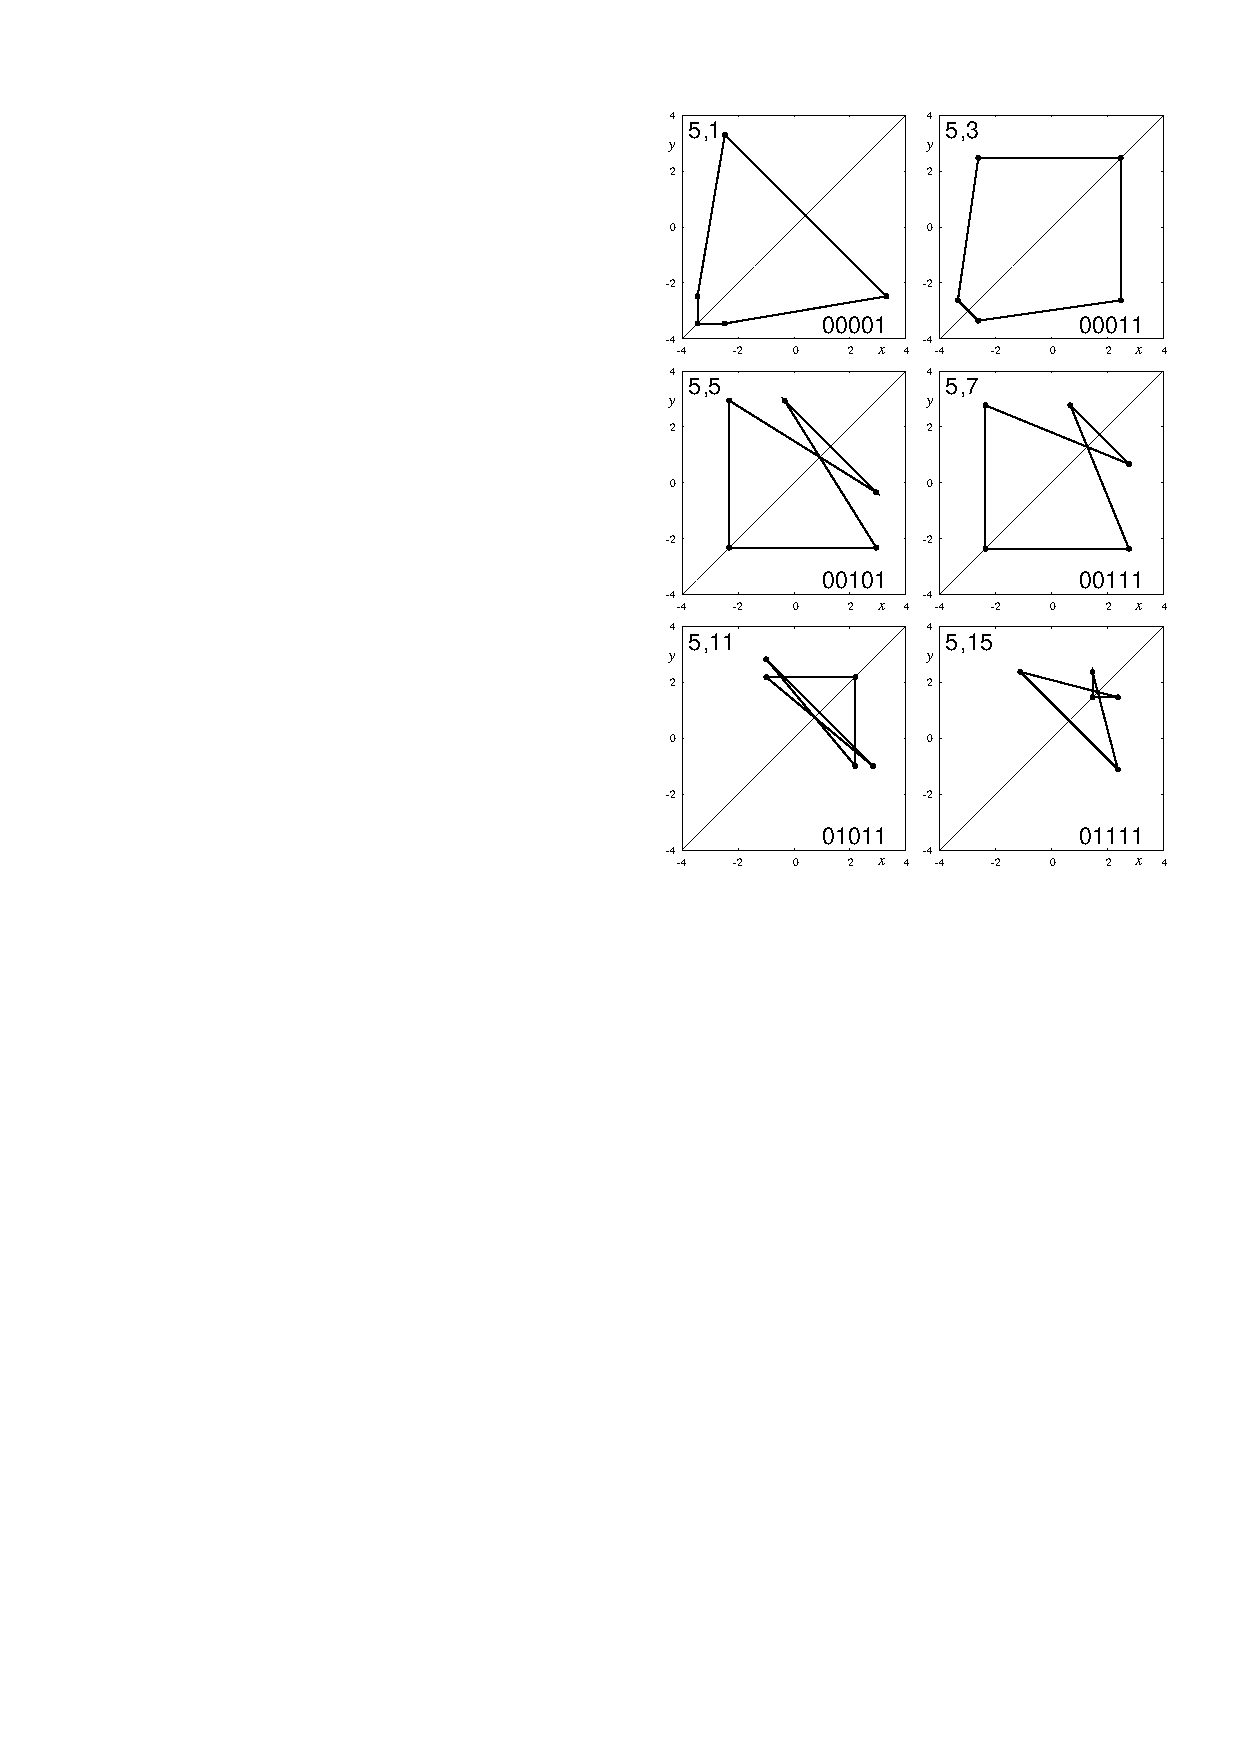
\includegraphics[width=0.60\textwidth]{EG05aCyc5}
}{}{
The 6 period-5 orbits are of Engler-Gallas class D (here called odd
period symmetric cycles $(o)$, see \refeq{reflSymOdd}): they are
symmetric under reflection across the diagonal, have a single point on
it, corresponding to 2 successive field values of an even-reflection pair.
Compare with the {\lattstate} plots of \reffig{fig:PChenlatt5cyc}.
The pairs 5,1 \& 5,3 and 5,1 \& 5,3 have an additional symmetry under
reflection and stretch (\PCedit{Predrag: what is that? I do not see it})
across the other diagonal.
%All six period-5 cycles are of class D:.
%They are symmetric under reflection about the diagonal shown. The pairs
%5,1 \& 5,3 and 5,5 \& 5,7 have an additional symmetry under reflection and
%stretch about the other diagonal.
%From \refref{EG05a}.
}{fig:EG05aCyc5}
%%%%%%%%%%%%%%%%%%%%%%%%%%%%%%%%%%%%%%%%%%%%%%%%%%%%%%%%%%%%%

                                                        \toCB
The problem of counting periodic orbits and its partitions is among the
first problems that one needs to address%
\rf{ChAnPi85,brucks,Lutzky88,Lutzky93,BLMS91,XH94,CheLou97,BriPer05}. For
the paradigmatic quadratic map it was addressed very early by
\HREF{https://en.wikipedia.org/wiki/Pekka_Myrberg} {Myrberg}, in what
appears to be one of the first applications of computers to
dynamics\rf{Myrberg58a,Myrberg58b,Myrberg59,Myrberg62,Myrberg63}. Apart
from counting orbits, he knew well how to exploit symbolic dynamics and
what was later named ``itineraries'' and ``kneading
sequences''\rf{MilThu88} to efficiently tabulate parameters with no less
than 11 digits of accuracy. The problem of counting orbits for the
{\HenonMap} was also addressed very early, in a pioneering work by
Sim{\'o}\rf{Simo79} using an approach centered in the strange attractor
creation/destruction.

The direct combinatorial problem of determining the partitions  $C_n$,
$D_n$, $N_n$  individually seems to be very hard. However there is an
efficient way of getting indirectly to them by counting the orbital
points lying on symmetry axis of the problem. This is what we do. The
approach is a nice application of enumerative combinatorics and the
number-theoretic Moebius inversion formula to a key problem in physics
and dynamical systems. Several complementary aspects of combinatorial
dynamics are discussed in \refref{AlLlMi00}.

\item[2021-02-18 Predrag]
\PCedit{Predrag: as the logistic map \refeq{Gallas20a:qm} is not invertible
map, I expect no information about the time reversal factorization from this
group of papers:}

Gallas\rf{Gallas18}
{\em Equivalence among orbital equations of polynomial maps}
 \arXiv{1809.05399}

Gallas\rf{Gallas20} {\em Orbital carriers and
inheritance in discrete-time quadratic dynamics} \arXiv{2008.01073}:

[...] may be all conveniently extracted from
just a single mathematical object, a polynomial called an
{\sl orbital carrier}, see for example \refeq{Gallas20a:S_5}.
All {\orbit}s may be encoded simultaneously by a single carrier,
with $p$ {\orbit} parameterized by the orbital sum $\sigma_p$.

recurrence

from  Pincherle's relation%\cite{Gautschi}
%\begin{equation}
% T_{\ell}(x) =  \left(\frac{x-\sqrt{x^2-4}}{2}\right)^{\ell}
%             + \left(\frac{x+\sqrt{x^2-4}}{2}\right)^{\ell},
%      \qquad \ell=0, 1, 2, \dots.
%\end{equation}


Sim{\'o}\rf{Simo79} {\em On the {H{\'e}non-Pomeau} attractor}
is a very fine early paper. Cite it in \Henon\ remark.
No mention of symmetry lines, though.

MacKay\rf{Bmack93} 1982 PhD thesis, published as
{\em Renormalisation in Area-preserving Maps} has a chapter on
reversible maps. Do cite in our paper(s).

The theory comes from deVogelaere\rf{DeVogelaere58} {\em On the structure
of symmetric periodic solutions of conservative systems, with
applications} (1958)

\end{description}
%%%%%%%%%%%%%%%%%%%%%%%%%%%%%%%%%%%%%%%%%%%%%%%%%%%%%%%%%%%%%%%%%%

\paragraph{{\Orbit}s and periodic points}

A \emph{periodic point} is a
solution $(x,\cl{})$, $x \in \reals^{d}$,
$\cl{} \in \integers$ of the {\em periodic orbit condition}
\index{periodic!orbit condition}
\beq
x = f^\cl{}(x)
\ee{COM:periodic}
for a given mapping $f$.
Each periodic point
$x=x_{p,i} \in p$
belongs to a \emph{time orbit}, a \emph{{\orbit}} $p$ of period $\cl{p}$,
and its  $\cl{p}$ distinct images
\[
f^k(x_{p,i})=x_{p,i+k}\,,\quad i+k \;\mbox{mod}\; \cl{p}
\]
are the successive periodic points
along the cycle.

A {\em {\orbit}}
\index{cycle!prime}
$p$ of period $\cl{p}$ is
a single traversal of the orbit.


We list the number of {\orbit}s up to length 10
for the 2-letter complete symbolic dynamics
in \reftabs{COM-t-mal-1}{COM-t-mal-78}.
% restore     (see \reftab{t-symm-3}).

%
% S = S_\asym^2 S_\sym S_b
% \refeq{EGfactorS}
\PC{27dec2004}{\reftab{COM-t-mal-78} derived from knead.tex} %, \refchap{c-knead}}
\PC{27dec2004}{extracted from smale.tex} %, \refchap{c-smale}}
%Predrag               27dec2004
%
%\index{H\'enon map}
%\index{map!H\'enon}
%For parameter $a$ sufficiently large the {\HenonMap} \refeq{eq2.1a} is
%another
%explicit example of a complete Smale horseshoe. %\rf{smale}.
%
% \noindent
% {\large\bf Hamiltonian {\HenonMap}}
% \\
% \PC{27dec2004}{included in  \refexam{exmp:HamHenonMap}}
% {[EG]}
%
% For definitiveness, in numerical calculations we shall fix here (arbitrarily)
% the stretching parameter value to $a=6$, a value large enough to guarantee
% that all roots of  $0=f^n(x)-x$ (periodic points) are real.
%
Consider the $n$-periodic point condition $0=f^n(x)-x$. This
polynomial of order $2^n$ has zeros at all
shorter, period $d$ {\orbit}s  if $d$ is a divisor of $\cl{}$.
Dividing those out, we arrive at the polynomial\rf{Milnor99}
\index{Moebius inversion}
\beq
Q_n(x) = \prod_{d|n}\left(f^d(x)-x\right)^{\mu({n / d})}
\,,
\ee{COMprimPoly}
 with $nM_n$ zeros corresponding to the $n$ periodic points
for each {\orbit} $p$ of period $\cl{p}=n$,
$
Q_n(x)= \prod_p P_p(x)
\,,
$
where the $n$th order polynomial
\beq
P_p(x) = \prod_{i\in p}(x-x_{p,i})=0
    \,,\qquad
\cl{p}=n
\ee{cycle-polyn}
has zeros at all periodic points in {\orbit} $p$.
Except for some values of $a$, at which bifurcations occur,
these are simple zeros.

The coefficients in the
expansion of \refeq{EGP} are symmetric polynomials in $x_i$,
all reducible to powers of the orbital sum  $\sigma_p$
\refeq{COMdef}, a {\orbit} $p$ invariant,
For example, the $x^{n-2}$ coefficient
\[
2 \sum_{i<j} x_i x_j =
    \sigma^2 - \sum_i x^2_i
    =
    \sigma^2 + 2\sigma - \cl{p}a
\]
can be expressed in terms of $\sigma^2$, $\sigma$ and $a$
\beq
P_p(x) = x^\cl{p} -\sigma_p x^{\cl{p}-1}
     + (\sigma^2 + 2\sigma - \cl{p}a)  x^{\cl{p}-2}
     + \cdots \pm (\sigma^\cl{p} \cdots)
\,.
\ee{COMPexp}
We refer to $\sigma$ as the ``center of mass'' of cycle $p$
(up to an overal prefactor of $1/\cl{p}$).

By cyclic invariance of periodic points in $p$, $\sigma_p$ is
invariant under $x \to f(x)$, so it is an intrinsic property of the
{\orbit} $p$, hence it can take at most  $M_n$ distinct values
corresponding to the $M_n$
{\orbit}s $p$ of period $\cl{p}=n$.

Endler and Gallas\rf{EG05} succeeded - after considerable algebra - in computing
explicitly the
$M_n$-th order polynomials
\beq
S_n(\sigma)=0
\,,
\ee{EGsigma}
\PC{27dec2004}{fill in the explanation}
for $\cl{p}\leq n$.
The $M_n$ root $\sigma=\sigma_p$
substituted into the $n$th order polynomial
\beq
P_n(x,\sigma_p,a) = \prod_{i\in p}(x-x_i)=0
\,,
\ee{EGP}
yields the $n$ periodic points $x=x_{p,i}$
belonging to the {\orbit} $p$ as the roots of $P_n(x,\sigma_p,a)=0$.
As the reduction of symmetric polynomial coefficients does not
rely on the shape of a given {\orbit} $p$,  $P_n$ has
the same form for all $\cl{p} = n$.
% and is parametrized by $\sigma$ and $a$.


\paragraph{Smale horseshoe}

Smale horseshoes and
symbolic dynamics labeling of the dynamics - it's really great, once you
get it, because the label tells you everything about the periodic point and
the cycle it belongs too. From \reftab{COM-t-mal-1}
 you can read off the shape and
symmetry of individual cycles, and the factorization of $S$ - at least the
highest power of $\sigma$ in each of the monic polynomials it factors into.

The \jacobianM\ %$\monodromy^n$
for the $n$th iterate of the Hamiltonian {\HenonMap} is
\index{Henon@H\'enon map!stability}
\beq
\monodromy^n(\xInit) = \prod_{m=n}^{1}
          \MatrixII{-2 x_m}{ -1 }
                   {1}  {0}
\,,\qquad x_m = f^{m}_1 (x_0,y_0)
\, .
\ee{COM:e_her}
\PC{27dec2004}{main text - explain the order of multiplication}
The determinant of the {\Henon} one time-step \jacobianM\ \refeq{COM:e_her}
is constant,
\beq
\det\monodromy = \ExpaEig_1 \ExpaEig_2 = 1
\ee{COM:HenDet}
so only one eigenvalue $\ExpaEig_1 = 1/\ExpaEig_2$
needs to be determined.


Iterating
$
   x_{n+1}=\flow{}{x_n} %\,,\quad x_0=\xInit
\,.
$ %ee{e-x-iter}
and checking the sign of $x_k$
associates a {\em temporally} ordered
topological itinerary $\Ssym{-m}\cdots \Ssym{-1}\Ssym{0}$
with a given trajectory,
\beq
   \Ssym{k} = \left\{
     \begin{array}{ll}
         1 & \mbox{if\ } x_k > 0 \\
         0 & \mbox{if\ } x_k < 0
     \end{array}
             \right.
 \,.
 \label{COM:e-symbol-df}
\eeq


\paragraph{Time reversal symmetry}
% Predrag               04apr2002
Under the time reversal
\refeq{COM:timeRevSymb}
the points in the  \topp\ for an \opres\ map are
symmetric across the diagonal $\gamma=\delta$.
Consequently the  periodic orbits appear either in dual pairs
$p=\Ssym{1} \Ssym{2} \Ssym{3} \ldots \Ssym{n}$,
$\overline{p}=\Ssym{n} \Ssym{n-1} \Ssym{n-2} \ldots \Ssym{1}$,
or are self-dual under time reversal,
$S_{p} = S_{\overline{p}}$.
% $\Ssym1 \Ssym2 \Ssym3 \ldots \Ssymn = \Ssymn \Ssym{n-1} \Ssym{n-2} \ldots \Ssym1$.

\PC{27dec2004}{insert this into the book}
For the \opres\ case
a self-dual cycle of odd period has at least one point (or odd number of
points) on the
symmetry diagonal. In particular, all fixed points lie on the symmetry
diagonal.

A self-dual cycle of even period has no, or even number of
points on the symmetry diagonal.

One distinguishes
three kinds of cycles: asymmetric cycles $\asym $,
symmetric cycles $\sym$ built by repeats of
irreducible segments $\symf$, and boundary cycles $b$.

\paragraph{Asymmetric cycles C} (`chiral' class):
A periodic orbits is not symmetric if
$\{x_\asym\} \cap \{{\bf R} x_\asym\} = \emptyset$, where
$\{x_\asym\}$ is the set of periodic points belonging to the cycle $\asym$.
Thus ${\bf R} $ generates a second orbit
with the same number of points and the same stability properties.

For this class of cycles for any $n$,
\beq
P_{\asym}(x,\sigma,a) = \prod^{p}(x-x_{\asym,i})
\ee{EGfactorA}
has $n$ distinct roots $\{x_{\asym,i}\}$.
The associated equation for is $C(\sigma)^2=0$.


\paragraph{Example}:
% Asymmetric pair:\\
Follow the successive periodic points in
the {\orbit} \cycle{0001011},
\reffig{COMcycles}\,(d);
then flip across the diagonal, reverse the direction along the
cycle, and you are now on
the {\orbit} \cycle{0001101}, the time reversed partner
of \cycle{0001011}.


\paragraph{Symmetric cycles, no boundary point N}
 (`non-diagonal' class):
A cycle $\sym$ is reflection symmetric if
operating with ${\bf R} $ on the set of
periodic points reproduces the set. The period of a symmetric cycle
is always even ($\nsym = 2 m$) and the mirror image of the
$x_\sym$ periodic point is reached by traversing the irreducible
segment $\symf$ of length $m$, $f^{m}(x_\sym) = {\bf R}  x_\sym $.
\beq
P_{N}(x,\sigma,a) = (x-x_{1}) (x-x_{2})^2 \cdots (x-x_{m})^2 (x-x_{m+1})
\ee{EGfactorN}
has $m+1$ distinct roots.
\beq
\sigma_p =  x_{1} + 2 x_{2} + \cdot + 2 x_{m} + x_{m+1}
\ee{COMdefN}

\paragraph{Example}:
Symmetric (or self-dual orbit):\\
Draw 4-cycles \cycle{0001} and \cycle{0111}.
They map into themselves under flip and time
reversal. That means that if you know 2 periodic points, the other 2 are
given by symmetry.

\paragraph{Even symmetric cycles, 2 boundary points  D}
 (`diagonal' class):
\beq
P_{D}(x,\sigma,a) = \prod^{p}(x-x_{\sym,i})^2
\ee{EGfactor2D}
has $\nsymf$ distinct roots.
\beq
\sigma_p = 2 \sum_{i}^{\nsymf} x_{p,i}
\ee{COMdef2D}

3 or more boundary points are not possible for {\orbit}s.

Cycle \cycle{0011} is an example of even-period boundary {\orbit} .
Two periodic points
$x_{1001}$,
$x_{0110}$
are on the symmetry diagonal, and reflection symmetry of the
remaining
$x_{0011}$,
$x_{1100}$ pair
forces a square-shaped trajectory in the $[x,y]$ plane,
see \reffig{COMcycles}:
\PC{27dec2004}{make into an exercise}
\[
\left[
\VectorII{x_{1001}}{x_{1001}},
\VectorII{-x_{1001}}{x_{1001}},
\VectorII{-x_{1001}}{-x_{1001}},
\VectorII{x_{1001}}{-x_{1001}}
\right]
\]
Hence $\sigma_{0011}=0$, and
\beq
      P_{0011}  =  (x^2-x_{0011}^2)^2
\,.
\label{COM:4-cycle}
\eeq
with  $x_{0011}=\sqrt{a}$. Note that this 4-cycle is more robust than the
2-cycle given in \refeq{COM:2-cycle}
- it exists for $a>0$, and is not the period-doubling relative
of the 2-cycle.

\paragraph{Odd symmetric cycles $n=2m+1$, 1 boundary point D }
 (`diagonal' class):
\beq
P_{B}(x,\sigma,a) = (x-x_{1})^2 \cdots (x-x_{m})^2 (x-x_{m+1})
\ee{EGfactor1B}
has $m+1$ distinct roots.
\beq
\sigma_p = 2 x_{1} + 2 x_{2} + \cdot + 2 x_{m} + x_{m+1}
\ee{COMdef1B}

\paragraph{Example}
Boundary cycles:\\
Draw 3-cycles \cycle{001} and \cycle{011}.
They have a point on the diagonal, indicated in
the table S.1.

The time reversal symmetry of the {\statesp} (this is true for
{\em all}
Hamiltonian time-reversible flows whose {\PoincSec} is symmetric
under $[q,p] \to [p,q]$ diagonal flip, not just polynomial mappings) implies
- but we need to cleanly explain it for this case
that $S_n(\sigma)$
{\em always} factorizes into form \refeq{EGfactorS}.
Endler and Gallas\rf{EG05} indeed observe that the polynomials
$S=S_n(\sigma)$ factorize into
product of polynomials over the above three kinds of cycles.

For each $n$, the $P_n(x,\sigma,a)$ polynomial should be written explicitly
for each of the 3 symmetry classes $[\asym,\sym,b]$. In particular,
for $P_{\sym}(x,\sigma,a)$ the factorization
over 1/2 of the {\statesp}
\beq
P_{\sym}(x,\sigma,a) = \left(\prod^{\symf}(x-x_{\symf,i})\right)^2
\ee{EGfactorP}
is expected, as exemplified by the 6-cycle
\reffig{COMcycles}\,(c).

\remark{``Center of mass'' puzzle.}{
The ``center of mass'' notions play important
role in a number of physical problems, such as:
(1) the periodic-orbit formulation of
the deterministic drift and diffusion
% restore      (\refchap{c-diffusion}),
(2) the kinematic dynamo
problem\rf{BCISV93,CGdynamo},
% appendLyapunov used to be appendApplic
% restore     (\refappe{c-appendLyapunov}),
and
(3) Sullivan's
formulation\rf{AACII,CCR,Pollicott91,Jiang}
of the Feigenbaum $\delta$ eigenvalue problem
in the period-doubling renormalization theory.

The ``center of mass'' puzzle for the cycles
listed in \reftab{gv:cycles} was first observed numerically
by G.~Vattay in \refref{BCISV93},
and was resolved by Endler and Gallas\rf{EG05}.
% Endler and Gallas\rf{EG05}
Their method of solution resembles the methods
earlier employed for quadratic polynomials (and their Julia sets) by
Brown\rf{Brown81}
    \PC{}{
    Brown\rf{Brown81} did all the right algebra for the logistic case.
    but computed approximate numbers rather than algebraic ones.
    }
and Stephenson\rf{Stephen1992A}.
Brown gives cycles up to length 6 for the logistic map,
employing symmetric functions of periodic points.
Hitzl and Zele\rf{HitZe85}
study the {\HenonMap} for cycle lengths  up to period  6.

All explicit values of periodic points
for the Hamiltonian {\HenonMap} displayed here
are taken from \refref{EG05}.
Method of \refref{EG05}
applies to cycles of polynomial maps only,
in this case the quadratic map.
        } %end \remark{
\index{center of mass}

\remark{Complete Smale horseshoe, Hamiltonian {\HenonMap}.}{
It was proved by Devaney and Nitecki\rf{Devaney79,StMeiss98}
that there is indeed a hyperbolic horseshoe when $a > 5+2\sqrt{5}$.
Numerical studies indicate that\rf{StMeiss98,SteDuMei99}
\beq
      a > 5.699310786700\cdots
\;.
\ee{COM:SterlHen}
    } % end \remark{Complete Smale horseshoe, Hamiltonian {\Henon}.}{


\section{Symmetries of the \topp}
\label{c-symbol-plane}
% 2021-02-15  Predrag if edits, return to appendFiniteGr

% restore     \cyclist

    \PC{2021-04-03}{
Moved to  here from ChaosBook \emph{appendFiniteGr}. Return once updated here.
    }
Depending on the type of dynamical system, the \topp\ might have
a variety of symmetries.
Under the time reversal
\beq
   \biinf{\Ssym{-2}\Ssym{-1}\Ssym{0}}{\Ssym{1}\Ssym{2} \Ssym{3}}
\to
   \biinf{\Ssym{3}\Ssym{2}\Ssym{1}}{\Ssym{0}\Ssym{-1} \Ssym{-2}}
\ee{COM:timeRevSymb}
the points in the  \topp\ for an \opres\ map are
symmetric across the diagonal $\gamma=\delta$, and
for the \orev\ case they are symmetric
with respect to the $\gamma=1-\delta$ diagonal.
Consequently the  periodic orbits appear either in dual pairs
$p=\Ssym{1} \Ssym{2} \Ssym{3} \ldots \Ssym{n}$,
$\overline{p}=\Ssym{n} \Ssym{n-1} \Ssym{n-2} \ldots \Ssym{1}$,
or are self-dual under time reversal,
$S_{p} = S_{\overline{p}}$.
% $\Ssym1 \Ssym2 \Ssym3 \ldots \Ssymn = \Ssymn \Ssym{n-1} \Ssym{n-2} \ldots \Ssym1$.
For the \opres\ case
a self-dual cycle of odd period has at least one point on the
symmetry diagonal. In particular, all fixed points lie on the symmetry
diagonal. Determination of such symmetry lines can be of considerable
practical utility, as it reduces some of the periodic orbit
searches to 1-dimensional searches.
	\PC{2021-03-24} {
create appendix
	chapter/appendCont.tex,
include
add JH Jan 18, 2008
{\em Desymmetrization of large spaces,
     thinking is extra price version}
% \label{sect:deSymmThink}
from
	halcrow/blog/TEX/symm.tex;
create
	Problems/exerAppCont.tex,
	Problems/soluAppCont.tex,
include
	halcrow/blog/TEX/zeghlache.tex;
create
	 chapter/refsAppCont.tex.
	}

\subsection{Symmetry lines}
\label{sect:SymmLines}
discuss symmetry lines

%%%%%%%%%%%%%%%%%%%%%%%%%%%%%%%%%%%%%%%%%%%%%%%%%%%%%%%%%%%%%%%
% \example{Symmetry lines of the standard map.}
\hfill \fastTrackExam{exam:StandMapSymmLin}
%%%%%%%%%%%%%%%%%%%%%%%%%%%%%%%%%%%%%%%%%%%%%%%%%%%%%%%%%%%%%%%

%%%%%%%%%%%%%%%%%%%%%%%%%%%%%%%%%%%%%%%%%%%%%%%%%%%%%%%%%%%%%%%
% \example{Symmetry lines of the cat map.}
\hfill \fastTrackExam{exam:CatMapSymmLin}
%%%%%%%%%%%%%%%%%%%%%%%%%%%%%%%%%%%%%%%%%%%%%%%%%%%%%%%%%%%%%%%


%%%%%%%%%%%%%%%%%%%%%%%%%%%%%%%%%%%%%%%%%%%%%%%%
\printbibliography[heading=subbibintoc,title={References}]

%%%%%%%%%%%%%%%%%%%%%%%%%%%%%%%%%%%%%%%%%%%%%%%%%%%%%%%%%%%%%
\newpage % REMOVE
  % examHenonMap.tex
% $Author: predrag $ $Date: 2021-12-24 01:25:20 -0500 (Fri, 24 Dec 2021) $

% Predrag extracted from                   2021-02-15
%                   ChaosBook.org
%%%%%%%%%%%%%%%%%%%%%%%%%%%%%%%%%%%%%%%%%%%%%%%%%%%%%%%
\example{{\HenonMap}.}{ \label{exam:HenonMap}
The map
\index{Henon@H\'enon map}\index{map!H\'enon}
\index{stretch \& fold}                                     \toCB
\bea
    x_{n+1}&=&1-ax^2_n+b y_n
        \continue
    y_{n+1}&=& x_n
\label{eq2.1b}
\eea
is a nonlinear 2\dmn\ map frequently employed in testing various hunches
about chaotic dynamics. Written as a  2nd-order inhomogeneous difference equation
(3-term recurrence relation), the {\henlatt} is
\beq
    x_{n+1}=1-ax^2_n+bx_{n-1} \, .
\ee{2-step}
An $(n+1)$-term recurrence relation is the discrete-time analogue
of an $n$th order differential equation, and it can always
be replaced by a set of $n$ 1-step relations.

% restore     The {\HenonMap} is the simplest map that captures the \stretchf\ dynamics
% restore     of return maps such as R\"ossler's, \reffig{f:RosslSect}.
% restore     It can be obtained by a truncation of a polynomial approximation
% restore     \refeq{approxPoinc} to a \PoincMap\ \refeq{approxPoinc} to second order.

%\index{map!once-folding}
%\index{once-folding map}
% restore     A quick sketch of the long-time dynamics of such a mapping
% restore     (an example is depicted in \reffig{FigHenonPer7}), is obtained
% restore     by picking an arbitrary starting point and
% restore     iterating \refeq{eq2.1a} on a computer.

Always plot the dynamics of such maps in the $(x_n,x_{n+1})$ plane,
rather than in the $(x_n,y_n)$ plane, and make sure that the ordinate and
abscissa scales are the same, so $x_n = x_{n+1}$ is the $45^o$ diagonal.
There are several reasons why one should plot this way: (a) we think of
the {\HenonMap} as a model return map $x_n \to x_{n+1}$, and (b) as
parameter $b$ varies, the attractor will change its $y$-axis scale, while
in the  $(x_n,x_{n+1})$ plane it goes to a parabola as $b\to0$, as it
should.
% restore     \exerbox{e-Henon-fixed}

% restore     As we shall soon see, {\po}s will be key to
% restore     understanding the long-time dynamics, so we also plot a typical
% restore     {\po} of such a system, in this case an unstable
% restore     period 7 cycle.
% restore     Numerical determination of such cycles will be
% restore     explained in \refsect{s-biham},
% restore     \PC{recheck this refsect}
% restore     and the periodic point labels
% restore     $0111010$, $1110100$, $\cdots$ in \refsect{s-smale}.
% restore            \jumpBack{exam:HenonMap}
    } %end \example{exam:HenonMap}
%%%%%%%%%%%%%%%%%%%%%%%%%%%%%%%%%%%%%%%%%%%%%%%%%%%%%%%

  % examHamHenonMap.tex called by examNewton.tex
% $Author: predrag $ $Date: 2021-05-04 15:35:29 -0400 (Tue, 04 May 2021) $

% Predrag                              2021-04-03
% called by \Chapter{newton}{17dec2020}{Hamiltonian dynamics}

%%%%%%%%%%%%%%%%%%%%%%%%%%%%%%%%%%%%%%%%%%%%%%%%%%%%%%%%%%%%%%%%%%
\example{{\Henlatt}.}{ \label{exam:HamHenonMap}
    \index{Henon@H\'enon map!Hamiltonian}                   \toCB
    \index{map!H\'enon!Hamiltonian}
    \index{map!Hamiltonian!H\'enon}
    \index{Hamiltonian!H\'enon map}
    \index{symplectic!H\'enon map}
    \index{area preserving!H\'enon map}
For $b=-1$ parameter value the {\HenonMap} \refeq{eq2.1a}  is the
simplest example of a nonlinear Hamiltonian map, a $2$\dmn\ {\opres},
area preserving map, often studied to better understand topology and
symmetries of \PoincSec s of 2-{\dofs} Hamiltonian flows.

We find it convenient\rf{EG05} to multiply \refeq{2-step} by
$a$ and absorb the $a$ factor into the definition the lattice field
$\field=a\,\ssp$.
This brings the Hamiltonian {\HenonMap} to the form
% analogous to the Fatou\rf{fatou} parabola parametrization:
\index{Henon@H\'enon map}
\bea
    \field_{n+1}&=&a-\field^2_n - p_n
                \continue
    p_{n+1}&=& \field_n
\,,
\label{Henlatt-eq2.1.0}
\eea
or, equivalently, the {\henlatt}
\refeq{EG05:ar_pres} 3-term recurrence relation of form
\beq
\field_{i+1} +\field_{i}^2 +\field_{i-1}=a  \, ,
\quad i=1,...,n_p
\,.
\label{Henlatt-2-step}
\eeq
We can write this as a
lattice field equation with lattice Laplacian \refeq{Box(2.1.1)}
\beq
  % \field_{n-1}-2\,\field_{n}+\field_{n+1}
\Box\,\field_{n}+(\field_{n}+2)\,\field_{n}\,=\, a
\,.
\ee{Henlatt-Lapl}
The field equation is nonlinear, with the
cubic potential \refeq{BWcubic}.

For definitiveness, in numerical calculations in examples
to follow we shall fix (arbitrarily)
the stretching parameter value to $a=6$, a value large enough to guarantee
that all roots of  $0=f^n(\ssp)-\ssp$ (periodic points) are real.
\exerbox{ex_birkhoff}
%\PC{link to next exer}
                                        \jumpBack{exam:HamHenonMap}
    } %end \example{HamHenonmap}
%%%%%%%%%%%%%%%%%%%%%%%%%%%%%%%%%%%%%%%%%%%%%%%%%%%%%%%%%%%%%%%%%%

%%%%%%%%%%%%%%%%%%%%%%%%%%%%%%%%%%%%%%%%%%%%%%%%%%%%%%%%%%%%%%%%%%
\example{{\Henlatt} fixed points.}{\label{exam:Henlatt-fixed}
% derived from ChaosBook {e-Henon-fixed}     Sept 6 2001
\index{Henon@H\'enon map!fixed points}
Since we are looking for fixed points $p_\stagn$ of
\refeq{Henlatt-eq2.1.0}, each successive step is the same as the
previous,
\[  \left( \begin{array}{c}
        \field_\stagn \\
        p_\stagn \\
        \end{array}\right)
         = \left(\begin{array}{c}
            a - \field_\stagn^2 -p_\stagn   \\
            \field_\stagn                 \\
            \end{array} \right)
\,.
\]
Thus there two fixed points, given by the roots of
the quadratic equation
$
\field^2 - 2\,\field - a = 0
\,,
$
\PC{2021-04-28}{agrees with Endler and Gallas\rf{EG05} $a=6$ values}
\bea
      \field_0 &=& -1 -\sqrt{1+a}
                        \continue
      \field_1 &=& -1 +\sqrt{1+a}
\,.
\label{Henlatt-2-cycle}
\eea

\PC{2021-04-28}{make into na exercise: Show that \refeq{Henlatt-2-cycle}...}
\cycle{01} periodic points are \refeq{COM:2-cycle}
\beq
      \field_{10}  =  { 1+ \sqrt{a-3} }
                        \,,\qquad
      \field_{01}  =  { 1- \sqrt{a-3} }
\,.
\label{Henlatt-exer:eq2}
\eeq


%\PC{link to next exam}
                                        \jumpBack{exam:Henlatt-fixed}
} %end \example{exam:Henlatt-fixed}
%%%%%%%%%%%%%%%%%%%%%%%%%%%%%%%%%%%%%%%%%%%%%%%%%%%%%%%%%%%%%%%

  % examHamHenonJacob.tex
% $Author: predrag $ $Date: 2021-09-02 23:44:14 -0400 (Thu, 02 Sep 2021) $

% Predrag extracted from                    2021-02-15
%                   ChaosBook.org
% based on                                  2021-04-27
%    \example{{\HenonMap} \jacobianM.}{ \label{exam:HenonJacob}
%    \example{Stability of cycles for maps.}{ \label{exam:cycStabMap}
%    siminos/kittens/cat.tex                2021-04-27
%%%%%%%%%%%%%%%%%%%%%%%%%%%%%%%%%%%%%%%%%%%%%%%%%%%%%%%%%%%%%%%%%%%%%%%%%%
\example{{\Henlatt} stability.}{ \label{exam:HamHenonJacob}
For the {\HenonMap} \refeq{Henlatt-eq2.1.0} the \emph{temporal evolution
\jacobianM} for the $n$th iterate of the map is the product of
consecutive  one time-step \jacobianMs\
\index{Henon@H\'enon map!stability}    \index{jacobian!H\'enon map}
\beq
\jMps^n(\field_0) =
\prod_{m=n}^{1}
          \MatrixII{-2\,\field_m}{-1}
                   {1}  {0}
\,,\qquad \field_m = \map^{m}_1 (\field_0,p_0)
\,.
\ee{Henlatt-e_her}
The decreasing order in the indices of the products in above formulas is
a reminder that the successive time steps correspond to multiplication
from the left,
$\jMps_p(\field_1)  = \jMps(\field_\cl{p})\cdots \jMps(\field_1)$.

The determinant of the {\Henon} one time-step \jacobianM\ in
\refeq{Henlatt-e_her} is a constant,
\beq
\det\jMps =
 1
\,,
\ee{Henlatt-HenDet}
so the map is Hamiltonian (symplectic) in the sense that it
preserves areas in the $[\field,p]$ plane.

The \FloquetM\ $\jMps_p$ for a {\orbit} $p$ of length
$\cl{p}$ of the {\HenonMap} \refeq{Henlatt-eq2.1.0} is evaluated by
picking any periodic point as a starting point, running once around a
{\orbit}, and multiplying the individual periodic point {\jacobianMs}
\refeq{Henlatt-e_her},
% restore     \ according to \refeq{jacoB}.
\index{Henon@H\'enon map!stability}
\beq
\jMps_p(\xInit) = \prod_{k=\cl{p}}^{1}
          \MatrixII{-2\field_k}{-1}
                   {1}  {0}
\,,\qquad \field_k \in \pS_p
\,,
\ee{Henlatt-Floq}
Once we have a {\po} of {\HenonMap}, we also have its \FloquetM.
Only the expanding eigen\-value $\ExpaEig_1=1/\ExpaEig_2$ needs to be
determined, as $\det\jMps = \ExpaEig_1 \ExpaEig_2=1$.

The {\em \jacobianOrb} is the $\delta/\delta\field_k$ derivative of the
{\henlatt} \refeq{Henlatt-2-step} 3-term recurrence relation
\bea
\jMorb_p &=&\sigma+2\,{\mathbb{X}}_p+\sigma^{-1}
\continue
 &=&
\begin{bmatrix}
2\,\field_0 & 1 & 0 & 0 & \dots & 0 & 1\\
1 & 2\,\field_1 & 1 & 0 & \dots & 0 & 0\\
0 & 1 & 2\,\field_2 & 1 & \dots & 0 & 0\\
\vdots & \vdots & \vdots & \vdots & \ddots & \vdots & \vdots\\
0 & 0 & \dots & \dots & \dots & 2\,\field_{\cl{}-2} & 1\\
1 & 0 & \dots & \dots & \dots & 1 & 2\,\field_{\cl{}-1}
\end{bmatrix}
\,,
\label{Henlatt-orbitJac}
\eea
where ${\mathbb{X}}_p$ is a diagonal matrix with $p$-{\lattstate} $\field_k$ in the
$k$th row/column, and the `$1$'s in the upper right and lower left corners
enforce the periodic boundary conditions.

The trace of the {\jacobianOrb} is twice the orbital sum\rf{Gallas20a}
\beq
\sigma_p = \sum_{i \in p} \field_{p,i}
\ee{Henlatt-COMdef}
% also \refeq{COMdef}
a \emph{prime} cycle $p$ \emph{invariant} that satisfies a
polynomial equation
${\mathbb S}_\cl{}(\sigma)=0$
of the order $\cl{p}$, the period of the cycle.
    \PC{2021-05-04}{Perhaps include the example \refeq{Gallas20a:S_5}?}

The two fixed points \refeq{Henlatt-exer:eq2} are hyperbolic for $a>3$,
with expanding eigenvalues
 % from \refeq{COM:eq3}.
\bea
      \ExpaEig_{0}  &=&  1+\sqrt{1+a}+ (1+a)^{1/4}\sqrt{\sqrt{1+a}+2}
                        \continue
      \ExpaEig_{1}  &=&  1-\sqrt{1+a}- (1+a)^{1/4}\sqrt{\sqrt{1+a}-2}
\,,
\label{Henlatt-COM:eq3}
\eea
\index{Henon@H\'enon map!fixed points}

%%%%% based on siminos/kittens/cat.tex                    2021-04-27 %%%%%
The action of the \henlatt\ {\jacobianOrb} can be hard to visualize,
as a period-2 {\lattstate} is a 2-torus,
period-3 {\lattstate} a 3-torus, \etc. Still, the {\fundPip} for the period-2
and period-3 {\lattstate}s, should suffice to
convey the idea. The {\fundPip} basis vectors \refeq{lattJac} are the
columns of $\jMorb$. The $[2\!\times\!2]$ {\jacobianOrb}
and its {\HillDet} follow from \refeq{Henlatt-2-cycle}
\beq
\jMorb =
 \left(\begin{array}{cc}
2\,\field_0 & 2 \\
          2 & 2\,\field_1
 \end{array} \right)
\,,\quad
\Det\jMorb = 4\,(\field_0\field_1-1)
           = -4\,(a-3)
\,.
\ee{Henlatt-catFundPar2}
% $( 1+ \sqrt{a-3} )( 1- \sqrt{a-3} )-1 = -a+3$
The resulting {\fundPip} shown in \reffig{fig:Henlatt-catCycJacob}\,(a).
Period-3
{\lattstate}s for $s=3$ are contained in the half-open {\fundPip} of
\reffig{fig:Henlatt-catCycJacob}\,(b),
defined by the columns of $[3\!\times\!3]$
{\jacobianOrb}
\beq
\jMorb =
\left(
\begin{array}{ccc}
2\,\field_0 & 1           & 1 \\
          1 & 2\,\field_1 & 1 \\
          1 & 1           & 2\,\field_2
\end{array}
\right)
\,,
\qquad
\Det \jMorb
    = 8\,\field_0\field_1\field_2-2\,(\field_0+\field_2+\field_3)+2
\,,
\label{Henlatt-catFundPar3}
\eeq
and for an period-$\cl{}$ {\lattstate},
    \PC{2021-05-04}{A guess, {\color{red}absolutely wrong - Fix!}}
\beq
\Det \jMorb
    = 2^\cl{}\field_0\field_1\field_2\cdots\field_{\cl{}-1}
    \,,\qquad \cl{}>3
\,.
\label{Henlatt-DetjMorb-n}
\eeq


% restore     \jumpBack{exam:HamHenonJacob}
% restore     \PC{explain \Henon\ = normal form in conjug.tex}
    } % end \example{exam:HamHenonJacob}
%%%%%%%%%%%%%%%%%%%%%%%%%%%%%%%%%%%%%%%%%%%%%%%%%%%%%%%%%%%%%%%%%%%%%%%%%%

  % examRevHenonMap.tex called by examNewton.tex
% $Author: predrag $ $Date: 2021-04-03 21:56:59 -0400 (Sat, 03 Apr 2021) $

% Predrag                              2021-04-03
% called by \Chapter{newton}{17dec2020}{Hamiltonian dynamics}

%%%%%%%%%%%%%%%%%%%%%%%%%%%%%%%%%%%%%%%%%%%%%%%%%%%%%%%%%%%%%%%%%%
%       former \section{Reversibility}          \label{s-Reversibility}
\example{Hamiltonian {\HenonMap}, reversibility.}{ \label{exam:RevHenonMap}
The {\HenonMap} \refeq{Ham-eq2.1.0} is reversible, with its inverse
interchanging the roles of $x$ and $y$:
\index{Henon@H\'enon map!reversible}
\index{map!reversible!H\'enon}
\index{reversible!H\'enon map}
\index{reversor}\index{involution}
\bea
    x_{n-1}&=& y_n
                \continue
    y_{n-1}&=& a-y^2_n - x_n
\, ,
\label{Ham-eq2.1.1}
\eea
hence the dynamics is symmetric in the  $[x,y]$ plane: a trajectory maps into a
trajectory under the flip across the $x=y$ diagonal
\beq
       \VectorII{y}{x} = R\VectorII{x}{y}
         =\MatrixII{0}{1}{1}{0} \VectorII{x}{y}
\ee{HenRev}
{\em and} the time reversal.
The reversor $R$ is {\orev}, $\det[\partial R]=-1$, and is an involution,
$R^2=\id$.
In other words, the Hamiltonian {\HenonMap} is conjugate to its inverse $f\circ
R=R\circ f^{-1}$, and can be factored into a pair of {\orev} involutions,
$f=(fR)\circ R=T\circ R$, with
\beq
       T\VectorII{x}{y} = \VectorII{x}{a-{x}^{2}-y}
\;.
\ee{HenRev2}
% Any image of a reversor is also a reversor.
% the full
% set $\{ (f^jR, f^jS) , j \in \integers\}$
% form an infinite set of reversors.
Equivalently, writing $f = S \circ (Sf) = S \circ U$, the reversor
\beq
       U\VectorII{x}{y} = \VectorII{a - y^2 - x}{y}
\ee{HenRev3}
factorizes the {\HenonMap} as $f = ST$.
                                        \jumpBack{exam:RevHenonMap}
    } %end \example{RevHenonMap}
%%%%%%%%%%%%%%%%%%%%%%%%%%%%%%%%%%%%%%%%%%%%%%%%%%%%%%%%%%%%%%%%%%

  % examStandMapSymmLin  called by examCycles.tex
% $Author: predrag $ $Date: 2021-04-10 21:40:23 -0400 (Sat, 10 Apr 2021) $

% Predrag                              2021-04-03
% called by \section{Examples} \label{exam:cycles}

%%%%%%%%%%%%%%%%%%%%%%%%%%%%%%%%%%%%%%%%%%%%%%%%%%%%%%%%%%%%%%%
\example{Symmetry lines of the standard map.}{ \label{exam:StandMapSymmLin}
    %\RA{Drop or modify and move to periodic orbit search as section/exercise/remark}
In practice the search for important classes of periodic orbits for the
standard map takes advantage of its remarkable symmetry: $A$ can be
written as the product of two {\em involutions},
$A = T_2 \cdot T_1$,
% $T_1$ and $T_2$
(involution means that the square of the map is the identity):
    \toRem{rem:symmLines}
\bea
% A &=& T_2 \cdot T_1
%        \continue
T_1 (x\,,\,y) &=&  (-x \,,\, y-k\sin x)
        \continue
T_2 (x\,,\,y) &=& (-x+y \,,\, y)
\, .
\label{StandMapInvol}
\eea
Now define symmetry lines ${\cal L}_1$ and ${\cal L}_2$ as the sets of fixed
points of the corresponding involution: ${\cal L}_1$ consists of the lines
$x=0, \pi$, ${\cal L}_2$ of $x=y/2 \,\,mod \, (2 \pi)$. There are deep
connections between symmetry lines and periodic orbits: we just give an
example with the following statement: if $(x_0,y_0) \in {\cal L}_1$ and
$A^M(x_0,y_0)\in {\cal L}_1$ ({\em i.e.} they are both fixed points of $T_1$),
then $(x_0,y_0)$ is a periodic point of period $2M$.
\PC{2021-04-03}{Bad notation - $M$ is \monodromyM}
As a matter of fact
\bea
A^{2M}(x_0,y_0)\,&=&\,A^{M-1}T_2T_1A^{M-1}T_2T_1(x_0,y_0) \nonumber \\
{\, \,} &=&\, A^{M-1}T_2A^{M-1}T_2(x_0,y_0)
\eea
by the fixed point property. Now the involution property implies
\beq
T_2A=T_1 \qquad \,\, AT_1=T_2
\eeq
and thus
\beq
AT_2AT_2\,=\,A T_1T_2\,=\,\matId
\eeq
and
\beq
A^PT_2A^PT_2\,=\,A^{P-1}T_2A^{P-1}T_2
\eeq
from which it easily follows that $(x_0,y_0)$ belongs to a $2M$ cycle.
                                        \jumpBack{exam:StandMapSymmLin}

(Continued in \refexam{exam:CatMapSymmLin}.)
    }%end \example{Symmetry lines of the standard map
%%%%%%%%%%%%%%%%%%%%%%%%%%%%%%%%%%%%%%%%%%%%%%%%%%%%%%%%%%%%%%%

  % examCatMapSymmLin.tex  called by examCycles.tex
% $Author: predrag $ $Date: 2021-05-04 19:02:36 -0400 (Tue, 04 May 2021) $

% Predrag                              2021-04-03
% called by \section{Examples} \label{exam:cycles}

%%%%%%%%%%%%%%%%%%%%%%%%%%%%%%%%%%%%%%%%%%%%%%%%%%%%%%%%%%%%%%%
\example{Symmetry lines of the cat map.}{ \label{exam:CatMapSymmLin}
~~~(Continued from \refexam{exam:StandMapSymmLin}.)
Instead of standard map, consider its linear relative, the
cat map, obtained by substituting $k\sin x \to Kx$ in \refeq{StandMapInvol}.
$A$ can now be
written as the matrix product of two {involutions},
$A = T_2\,T_1$,
\bea
% A &=& T_2 \cdot T_1
%        \continue
T_1 (x\,,\,p) =  (-x \,,\, p-K x)
&\Rightarrow& T_1 =
         \MatrixII{-1 }{0}
				  {s-2}{1}
        \continue
T_2 (x\,,\,p) = (-x+p \,,\, p)
&\Rightarrow& T_2 =
         \MatrixII{-1}{1}
				  { 0}{1}
        \continue
&\Rightarrow& A =
         \MatrixII{s-1}{1}
				  {s-2}{1}
\,.
\label{CatMapInvol}
\eea
$T_1$ and $T_2$ are
involutions as their squares are the identity.
We have substituted $K=-s+2$, where ${s}=\tr{A}$.

\PC{2021-04-10}{complete the rewrite here.}
Now define symmetry lines ${\cal L}_1$ and ${\cal L}_2$ as the sets of fixed
points of the corresponding involution: ${\cal L}_1$ consists of the lines
$x=0   \mod 1$, ${\cal L}_2$ of $p=2x$. There are deep
connections between symmetry lines and periodic orbits: we just give an
example with the following statement: if $(x_0,p_0) \in {\cal L}_1$ and
$A^M(x_0,p_0)\in {\cal L}_1$ ({\em i.e.} they are both fixed points of $T_1$),
then $(x_0,p_0)$ is a periodic point of period $2M$.
As a matter of fact
\bea
A^{2M}(x_0,p_0)\,&=&\,A^{M-1}T_2T_1A^{M-1}T_2T_1(x_0,p_0) \nonumber \\
{\, \,} &=&\, A^{M-1}T_2A^{M-1}T_2(x_0,p_0)
\eea
by the fixed point property. Now the involution property implies
\beq
T_2A=T_1 \qquad \,\, AT_1=T_2
\eeq
and thus
\beq
AT_2AT_2\,=\,A T_1T_2\,=\,\matId
\eeq
and
\beq
A^PT_2A^PT_2\,=\,A^{P-1}T_2A^{P-1}T_2
\eeq
from which it easily follows that $(x_0,p_0)$ belongs to a $2M$ cycle.

I see no $\jMorb=\transp{\tilde{\jMorb}}\tilde{\jMorb}$ factorization in
style of \refeq{tildejMorb}  % copy of PC(1.2.11)}

                                        \jumpBack{exam:CatMapSymmLin}
    }%end \example{Symmetry lines of the standard map
%%%%%%%%%%%%%%%%%%%%%%%%%%%%%%%%%%%%%%%%%%%%%%%%%%%%%%%%%%%%%%%


  % siminos/spatiotemp/Problems/exerHamHenonCyc.tex called by Henon.tex
% $Author: predrag $ $Date: 2021-10-15 15:55:44 -0400 (Fri, 15 Oct 2021) $

\Problems{exerFixed}{14oct2021}

%%%%%%%%%%%%%%%%%%%%%%%%%%%%%%%%%%%%%%%%%%%%%%%%%%%%%%%%%%%%%%%
% Predrag                   27apr2021, 14oct2021
% Predrag                   26oct2014
\exercise{Inverse iteration method for a {\Henon} repeller.}{
                \label{exer:HamHenonCyc}
\index{inverse!iteration, Hamiltonian repeller}
\index{iteration!inverse!Hamiltonian repeller}
\index{periodic!orbit!Hamiltonian repeller}
\index{Hamiltonian!repeller, periodic orbits}

%%%%%%%%%%%%%%%%%%%%%%%%%%%%%%%%%%%%%%%%%%%%%%%%%%%%%%%%%%
\begin{table}
\caption{\label{gv:cycles}
 All {\po}s up to $\cl{}=6$
for the Hamiltonian {\HenonMap} repeller
%\refeq{e:pere}
\refeq{pere}
with $a=6$.
Listed are the cycle itinerary, its expanding eigenvalue $\ExpaEig_p$,
and its ``center of mass.'' The ``center of mass'' is listed because
it turns out that it is often a simple rational
or a quadratic irrational.
All {\orbit}s up to topological length $n=20$
have been computed.
    }
\renewcommand{\arraystretch}{0.7}
\noindent
{ \small
\begin{tabular}{lrr}
% \setdec 00.00000
% V                    &\dec 1.04323   &\dec 0.48474   &  5&     -1 \\
~~~~$p$~~~~ & $\ExpaEig_p$~~~~~~~~~~~~
          &    $\sum \ssp_{p,i}~~~~~$ \\
    \hline
0 & 0.715168$\times 10^1$ & -0.607625 \\
1 &-0.295285$\times 10^1$ &  0.274292 \\
%   \hline
10 &-0.989898$\times 10^1$ &  0.333333 \\
%   \hline
100 &-0.131907$\times 10^3$ & -0.206011 \\
110 & 0.558970$\times 10^2$ &  0.539345 \\
%   \hline
1000 &-0.104430$\times 10^4$ & -0.816497 \\
1100 & 0.577998$\times 10^4$ &  0.000000 \\
1110 &-0.103688$\times 10^3$ &  0.816497 \\
%   \hline
10000 &-0.760653$\times 10^4$ & -1.426032 \\
11000 & 0.444552$\times 10^4$ & -0.606654 \\
10100 & 0.770202$\times 10^3$ &  0.151375 \\
11100 &-0.710688$\times 10^3$ &  0.248463 \\
11010 &-0.589499$\times 10^3$ &  0.870695 \\
11110 & 0.390994$\times 10^3$ &  1.095485 \\
%   \hline
100000 &-0.545745$\times 10^5$ & -2.034134 \\
110000 & 0.322221$\times 10^5$ & -1.215250 \\
101000 & 0.513762$\times 10^4$ & -0.450662 \\
111000 &-0.478461$\times 10^4$ & -0.366025 \\
110100 &-0.639400$\times 10^4$ &  0.333333 \\
101100 &-0.639400$\times 10^4$ &  0.333333 \\
111100 & 0.390194$\times 10^4$ &  0.548583 \\
111010 & 0.109491$\times 10^4$ &  1.151463 \\
111110 &-0.104338$\times 10^4$ &  1.366025
\end{tabular}
} %end { \small
\end{table}
\renewcommand{\arraystretch}{1.0}
%%%%%%%%%%%%%%%%%%%%%%%%%%%%%%%%%%%%%%%%%%%%%%%%%%%%%%%%%%

                                                \toCB
    \PC{14oct2021}{Return to ChaosBook eventually}
    \PC{27dec2004}{give the center of mass paper reference somewhere}
%
Consider the  {\HenonMap} \refeq{eq2.1a}
for the area-preserving (``Hamiltonian'') parameter value $b=-1$.
The coordinates of a {\po} of
length $n_p$ satisfy the  equation
\index{Henon@H\'enon map!cycles}
\beq
\ssp_{p,i+1}+\ssp_{p,i-1}=1 -  a \ssp_{p,i}^2 \, ,
\quad i=1,...,n_p
\,,
\label{pere}
\eeq
with the periodic boundary condition
%$\ssp_{p,n_p +1}=\ssp_{p,1}$ and
$\ssp_{p,0}=\ssp_{p,n_p}$.
Verify that the itineraries and the stabilities of the short
{\po}s for the {\Henon} repeller \refeq{pere}
at $a=6$ are as listed in \reftab{gv:cycles}.

{\bf Hint}: you can use any cycle-searching routine you wish, but for the
complete repeller case (all binary sequences are realized), the cycles
can be evaluated by inverse iteration
$\ssp_{p,i}^{(m+1)}\to\ssp_{p,i}^{\infty}=\ssp_{p,i}$, estimating
the midpoint by square-root
of \refeq{pere}
\beq
\ssp_{p,i}^{(m+1)}=\sign{p,i}
     \sqrt{\frac{1-\ssp_{p,i+1}^{(m)}-\ssp_{p,i-1}^{(m)}}{a}}
\,.
\ee{GVinver}
Here $\sign{p,i}$ are the
signs of the corresponding periodic point coordinates,
$\sign{p,i}=\ssp_{p,i}/|\ssp_{p,i}|$,
% and $i=1,...,n_p$
related in the obvious way to desired \po's binary itinerary,
\beq
\sign{i}+1=2\,\Ssym{i}\,,\quad \Ssym{i}\in\{0,1\}
\,.
\ee{henonSigns}
see \reffig{fig:PChenlatt5cyc}.
%
\hfill G.~Vattay
    } % end \exercise{A Hamiltonian repeller}
%%%%%%%%%%%%%%%%%%%%%%%%%%%%%%%%%%%%%%%%%%%%%%%%%%%%%%%%%%%%%%%

%%%%%%%%%%%%%%%%%%%%%%%%%%%%%%%%%%%%%%%%%%%%%%%%%%%%%%%%%%%%%%%
\exercise{``Center of mass'' puzzle.}{\label{e:CenterOfMass}
% \tangent
Why is the ``center of mass,'' tabulated
in \refexer{exer:HamHenonCyc}, often a rational number?
\index{center of mass}
%    \else listed in \reftab{gv:cycles},
    } % end \exercise{``Center of mass'' puzzle
%%%%%%%%%%%%%%%%%%%%%%%%%%%%%%%%%%%%%%%%%%%%%%%%%%%%%%%%%%%%%%%

    \ProblemsEnd

  % soluHamHenonCyc.tex
% $Author: predrag $ $Date: 2021-10-14 11:00:27 -0400 (Thu, 14 Oct 2021) $

\Solution{Henon}{soluFixed}{26oct2014}{{\HenonMap}}
% Predrag                                       26oct2014
%       from ChaosBook soluFixed

%%%%%%%%%%%%%%%%%%%%%%%%%%%%%%%%%%%%%%%%%%%%%%%%%%%%%%%%%%%%%%%%%%%%%%%
\solution{exer:HamHenonCyc}
         {Inverse iteration method for a Hamiltonian repeller.}{
\index{inverse!iteration, Hamiltonian repeller}
\index{iteration!inverse!Hamiltonian repeller}
\index{periodic!orbit!Hamiltonian repeller}
\index{Hamiltonian!repeller, periodic orbits}
For the complete repeller case (all binary sequences are realized),
the cycles can be evaluated variationally, as follows.
According to \refeq{eq2.1a},
% (\ref{times}),
the coordinates of a periodic orbit of
length $n_p$ satisfy the  equation
                                \toCB
\beq
\ssp_{p,i+1}+\ssp_{p,i-1}=1 -  a \ssp_{p,i}^2 \, ,
\quad i=1,...,n_p
\,,
\label{e:pere}
\eeq
with the periodic boundary condition
%$\ssp_{p,n_p +1}=\ssp_{p,1}$ and
$\ssp_{p,0}=\ssp_{p,n_p}$.

In the complete repeller case, the {\HenonMap} is a realization
of the Smale horseshoe, and the symbolic dynamics has a very simple
description in terms of the
binary alphabet  $\epsilon \in \{ 0,1 \}$,
$\epsilon_{p,i}=(1+S_{p,i})/2$, where $S_{p,i}$ are the
signs of the corresponding periodic point coordinates,
$S_{p,i}=\ssp_{p,i}/|\ssp_{p,i}|$.
We start with a preassigned sign sequence
$S_{p,1},S_{p,2}, \dots, S_{p,n_p}$, and a
good  initial guess for the coordinates $\ssp_{p,i}'$.
Using the inverse of the equation (\ref{pere})
\[
\ssp_{p,i}''=S_{p,i}\sqrt{\frac{1-\ssp_{p,i+1}'-\ssp_{p,i-1}'}{a}}
\,\quad i=1,...,n_p
\]
we converge iteratively, at exponential rate, to the desired
periodic points $\ssp_{p,i}$. Given the periodic points, the cycle
stabilities and periods are easily computed using
\refeq{Henlatt-e_her}. The itineraries and the stabilities of the short
periodic orbits for the {\Henon} repeller \refeq{e:pere} for
$a=6$ are listed in \reftab{gv:cycles}; in actual
calculations all {\orbit}s up to topological length $n=20$
have been computed.
%
\hfill G.~Vattay
} % end \solution{A Hamiltonian repeller}
%%%%%%%%%%%%%%%%%%%%%%%%%%%%%%%%%%%%%%%%%%%%%%%%%%%%%%%%%%%%%%%%%%%%%%%


\ChapterEnd % formatted for ChaosBook.org
